\documentclass[12pt]{article}

\pdfminorversion=4

\usepackage[utf8]{inputenc} %unicode support

\usepackage{amsmath}
\usepackage{amssymb}
%\usepackage{pdfpages}
\usepackage{gensymb}
\usepackage{graphicx}
\usepackage{epstopdf}
\usepackage{color}
\usepackage[margin=1in]{geometry}
\usepackage{times,mathptmx}
\usepackage{longtable}

% Bold the 'Figure #' in the caption and separate it with a period
% Captions will be left justified
\usepackage[labelfont=bf,labelsep=period,justification=raggedright]{caption}

% Use the ACS provided bibtex style
\bibliographystyle{plain}
%\bibliographystyle{acs}
\usepackage{cite}

% Remove brackets from numbering in List of References
\makeatletter
\renewcommand{\@biblabel}[1]{\quad#1.}
\makeatother


% definition of \customlabel, which is used to label supplementary figures and tables
\makeatletter
\newcommand{\customlabel}[2]{%
\protected@write \@auxout {}{\string \newlabel {#1}{{#2}{}}}}
\makeatother


\begin{document}


\title{Large-scale analysis of post-translational modifications in \emph{E. coli} under glucose-limiting conditions over 2 weeks}

\author{Viswanadham Sridhara$^1$, Colin Brown$^{2}$, Daniel R. Boutz$^{2,3}$, Maria D. Person$^{4}$,\\
Jeffrey E. Barrick$^{1,2,3,5}$, Edward M. Marcotte$^{1,2,3,5}$, and Claus O. Wilke$^{1,2,3,6}$}
\maketitle

\noindent
$^1$Center for Computational Biology and Bioinformatics, The University of Texas at Austin, Austin, TX, USA\\
$^2$Institute for Cellular and Molecular Biology, The University of Texas at Austin, Austin, TX, USA\\
$^3$Center for Systems and Synthetic Biology, The University of Texas at Austin, Austin, TX, USA\\
$^4$College of Pharmacy, The University of Texas at Austin, Austin, TX, USA\\
$^5$Department of Molecular Biosciences, The University of Texas at Austin, Austin, TX, USA\\
$^6$Department of Integrative Biology, The University of Texas at Austin, Austin, TX, USA\\


\begin{abstract}
How do the post-translational modifications [PTMs] change over time during microbial growth under nutrient limiting conditions? We sought to answer this question using \emph{E. coli} grown under glucose starvation conditions. We generated mass-spectrometry based proteomics data at 9 different time points ranging from exponential to long stationary phases i.e., upto 2 weeks. We then ran MODa, a program that identifies peptide-spectral matches, on this data for an unrestricted search of PTMs. There were several interesting observations in this MODa analysis. First, we show that the amount of modified protein seems to be constant, occuring approx. 30\%, at all the 9 time points. Second, we show that acetylations, especially n-term acetylations increase over time and we were able to identify new protein targets that gets acetylated. Third, we show that sulfoxide reductases fix MetSO to Met during stationary phase, protecting \emph{E. coli} from oxidative damage. Fourth, we found that phosphorylations, even though less abundant, increase under these starvation conditions in \emph{E. coli}. Finally, we found some novel post-translational modifications in this data, a frequent one being 39 dalton mass-shift on Isoleucine on exonuclease ABC subunit C.
\end{abstract}

% keywords: post-translational modifications

\section{Introduction}

Mass-spectrometry based proteomics \cite{Lamondetal2012} offers a unique way to characterize different post-translational modifications [PTMs] associated with proteins. PTMs are key in determining protein function, localization and regulation. Hundreds of PTMs are known \emph{in vivo}, however most of the current studies focus on identifying only few PTMs from mass-spec data. This is both because of computational limitations as well as the inefficiency of enrichment techniques to characterize or identify all PTMs. However with the improvement of search algorithms for an unrestricted search of PTMs, identifying multiple PTMs in \emph{tandem} has become a possibility. In this work, we used MODa \cite{Naetal2012}, a naive based spectral alignment algorithm to do an unrestricted search of PTMs from mass-spectrometry based proteomics data in \emph{E. coli} REL606 strain.

In a typical mass-spectrometry based proteomics experiment, proteins are first digested into peptides and then the sample is enriched for any PTMs of interest. This sample is then analyzed by mass-spectrometry. Peptide search algorithms are then run on this mass-spectrometry data to computationally identify peptides and PTMs associated with it. These search algorithms generally fall into 3 categories: (1) Sequence or database search algorithms, (2) de novo sequence search and (3) Hybrid approach that is a mixture of partial de novo search followed by a database search. Most of the current search algorithms such as Mascot\cite{Perkinsetal1999}, Sequest \cite{Engetal1994}, OMSSA \cite{Geeretal2004}, X!Tandem \cite{CraigBeavis2004} search for only few variable modifications, i.e., oxidation of methionine etc or a small targeted list of PTMs. This technique of restricted search reduces the size of the database to search and hence alleviates lot of computational limitations \cite{McHughArthur2008}. Even though few of these algorithms report an option to do an unrestricted search, there are very few studies that reported an unrestricted search of PTMs using these algorithms. However, recently, software for unrestricted search of PTMs is starting to be available. MODa \cite{Naetal2012} is one such unrestricted search engine, along with others such as TagRecon\cite{Dasarietal2010} and Byonic \cite{Bernetal2012}. We used MODa, a spectral alignment algorithm that uses dynamic programming to identify small mass-tags and then join them reporting the delta masses between these mass tags. MODa is being used frequently to do an unrestricted search and identify novel PTMs. Some of the studies that used MODa either looked at particular PTM \textbf{WHAT} \cite{Kimetal2014}, or looked at wider coverage of PTMs such as \cite{Liuetal2013}. Here we used MODa, first to do an unrestricted search to identify frequently occuring mass-shifts and focussed on the PTMs that seem abundant in this data or being reported to be critical with \emph{E. coli}. 

%Mapping the entire proteome involves mapping all the post-translational modifications on the proteins. This is a challenging goal, given the enrichment techniques for PTMs along with the computational search algorithms to identify these PTMs.
%In the last decade, however there has been lot of effort to improve search algorithms to increase the coverage of PTMs i.e., using unrestricted approaches instead of traditional search, where a guessed list of only handful PTMs is provided beforehand.

In our current work, we generated mass-spectrometry data for \emph{E. coli} grown under glucose limiting conditions. As shown in many studies \cite{Soaresetal2013}\cite{Soufietal2015}, \emph{E. coli} grown under these nutrient limiting conditions generally behave differently at different phases of their growth i.e., during exponential and stationary phases. During the stationary phase, stress response proteins act because of the conditions caused by limiting nutrients, change in pH value, accumulation of toxic substances in the flasks etc \cite{Nystrom2004}. Most of the studies till now focussed on identifying proteins that were differentially expressed under these different conditions of growth. However, there are very few studies that looked at the PTM level information during such nutrient-limiting growth. In one study that looked at phosphoproteome \cite{Soaresetal2013}, the number of phosphorylation sites as well as their occupancy levels have been shown to increase from exponential to stationary phase, suggesting likely role of this PTM in stationary phase. In the same study, the authors showed that protein abundance of SspA, a stress protein seemed to be constant during the time course of growth, while the number of phosphorylated sites on the same protein increased. This clearly suggests PTM level quantitation to be key to understand how \emph{E. coli} responds to stress. In a recent study by Soufi et. al., \cite{Soufietal2015}, the authors investigated the \emph{E. coli} proteome dynamics at 7 different time points (exponetial to extended stationary phases) of growth. They looked at protein abundances, copy numbers and also investigated briefly on PTMs. In their work, the authors looked at the pair-wise correlation of the PTMs identified in different stages of growth. Even though the authors looked at few PTMs, they did not do PTM level quantitation. Our work is focussed not only on doing an unrestricted search of PTMs, but understanding the PTM levels during the exponential and long-stationary phases of \emph{E. coli} growth.

%In another study, in \emph{acinetobacter baumannii} by the same group \cite{Soaresetal2010}, the oxidative stress has been shown to be compensated by the \emph{E. coli} machinery at the later stages of growth i.e., stationary phase compared to the early exponential phase. This itself suggests that PTM level analysis is necessary to understand the response of organisms to environmental and other disturbances.
%\textbf{in ABOVE para, Not clear what "compensated by the E. coli machinery at later stages" means...is the point that A.b. regulates SspA by conrolling protein level?  What does the E. coli machinery have to do with this?}

Few other studies of PTMs focussed on multiple PTMs \cite{Guptaetal2007}, but they looked at only one "snapshot" of interest i.e., a single time point during the growth or used information from a larger database of processed mass-spectrometry data. Our focus is to understand how these PTMs dynamically change during their growth in a single experiment. Since it has already been shown that during different phases of growth, different proteins will be expressed, a "snapshot" of PTM analysis does not provide a clearer picture on the significance or the function associated by these PTMs. Our current work of using multiple time points during the growth curve or looking at multiple "snapshots" along with an unrestricted search of PTMs provides a holistic view of proteome function. 

%Few sites have been previously shown to be modified by different PTMs depending on the circumstances. So, analyzing multiple PTMs in tandem is necessary to understand behavior of microbes under different conditions. Here, we argue that we need a comprehensive analysis of PTMs at different time points to understand the PTM level response. 

%Our earlier work using the protein, mRNA, lipid and metabolite level information at different phases in growth suggested the significance of such comprehensive analysis. However, we did not focus our earlier work at PTM level, but instead analyzed the protein abundances. Here, we did an unrestricted search to identify most of the PTMs and at 9 different time points during the exponential and long-stationary phases lasting upto 2 weeks.

\section{Results}

\subsection{Running MODa on \emph{E. coli} proteome}
Post-translational modifications, in most cases, determine the specific function of the protein. Identifying all the PTM combinations or the set of PTMs associated with all the proteins (i.e., entire proteome) is limited by experimental enrichment techniques for PTMs as well as computational limitations. The current analysis of \emph{E. coli} dataset is not enriched for any PTMs. This means that this dataset is suitable for hunting for different kinds of PTMs, instead of focussing on particular PTMs. Most of the current studies focus on a single PTM coverage, such as generally done in phosphoproteomics studies, glycosylation studies or acetylation studies, where the sample is enriched for a particular PTM. 

We have mass-spectrometry data at 9 different points of the OD600 curve (see Suppl Figure S1). At each time point, there were 3 biological replicates. We then used MODa on each of these data sets to identify the PTM level information. MODa is a sequence search algorithm that takes as an input mass-spectrometry data and identifies peptides and PTMs associated with the proteins. MODa is a naive based search algorithm that uses an unrestricted approach to find the post-translational modifications in the data. The parameters used with MODa is described in detail in the methods section of the paper. In brief, MODa uses multiple short sequence tag information in the spectra along with a dynamic programming approach to identify the peptide hits along with their protein identifiers. The use of multiple tags reduces both the database size and the false positives. MODa outputs 2 data files that we used in our analyses (1) it outputs the frequency of the mass-shifts on different amino-acids along with N- and C- term of the peptides, (2) it outputs peptide level information like most of other search engines. Once we have the MODa search results, we asked the following questions: (a) How much of the proteome is modified? (b) How do these modifications change over time? (c) Is there any biological relevance associated with the temporal change of a particular PTM? (c) Can we find any novel modifications in this \emph{E. coli} data? 

%The mass-spectrometry data gathered at the 9 time points is then searched for PTMs using MODa, a naive based spectral alignment search algorithm, for peptide identifications. At each of these 9 time points, we gathered data for 3 biological replicates. Unlike most of the other peptide identification search algorithms, MODa requires range of mass for PTM identification. So, for our analysis we used a range of -200 to 200 Da which is typical to this search engine. MODa is a multi-blind algorithm i.e., there is no restriction on the  number of PTMs identified on a single peptide. However previous studies have shown better sensitivity of the algorithm with the use of 1 mod per peptide. We used 1 mod per peptide for most of the analysis, however we compared our results with using 2 mods per peptide too.

%(d) Can we explain the pattern of the PTMs over time using other diverse kinds of data such as RNA-seq? In this project, we also collected mRNA via RNA-seq, lipid profiles and metabolic fluxes using mass-spec methods. We went back and compared our proteomics data with these other kinds of data for further validation, wherever necessary.

\subsection{Modified \emph{E. coli} proteome}
First, we are interested in identifying the amount of proteome modified. Since we have data at each of the 9 time points i.e., from exponential to long-stationary phases, we plotted the total frequency of all PTMs at each of these time points. For this, we simply calculated the percentage of the total number of modified peptide spectral matches (PSMs) at each time point. We used 1 standard error to plot the variation within 3 biological replicates.

Figure~\ref{fig:ModifiedPTM} shows the total percent of the peptide-spectral matches on the y-axis and the time from OD600 plot on the x-axis. It is clear that the amount of spectra that is modified stays approx. at 30\% during all the phases of the growth. Most of the previous studies on identifying multiple tandem PTMs looked at a "snapshot" of the proteome, instead of looking at different phases during the growth. We then looked at the coverage of the proteome at these time points. The number of proteins identified at each of these 9 time points are 2227, 2246
,2278, 2251, 2306, 2342, 2298, 2234 and 2193 respectively. The number of identifications are a bit lower when compared to our previous analysis using Sequest \cite{Houseretal2015}. However MODa is an algorithm that is more widely used to unravel new PTMs than to increase the protein coverage. We considered all the peptide spectral matches i.e., one-hit wonders too. Later, when we use the data to identify the protein targets for different PTMs, we included a strict criteria of including proteins that have at least 2 peptide hits. This resulted in 1861, 1822, 1857, 1839, 1864, 1892, 1866, 1813 and 1758 protein identifications at each of the 9 time points analyzed in this study.
%(Cite some studies, for example Soufi et al and other papers they cited?)
%However note that a modification could be a mutation or a post-translational modification.

\subsection{Mapping mass-shifts to post-translational modifications}

We next looked at the distribution of the mass-shifts or PTMs at each time point of the growth curve i.e., what PTMs are present at a given time point and how does it change over time? MODa outputs mass-shifts in integer masses in the peptide hits. A mass-shift indicates either a PTM or a substitution compared to the reference database. The mass-shifts are then converted to PTMs using UNIMOD database, as described in methods section. For example, we know that +16 Dalton shift on any amino acid is most likely the oxidation. When we looked at the UNIMOD PTM list, we did see that this is oxidation, generally shown to occur on few amino acids such as cysteine, methionine etc. We did not limit our analysis to frequently occuring mass-shifts, but also focussed on well known PTMs, and novel mass-shifts that were not characterized earlier. However, we did not investigate into mutations and this will be a topic we will look in the future as this is a possibility with MODa output.

Even though the total amount of modified proteome is mostly constant ~30\%, the content of PTMs at each time point vary during different phases of growth i.e., a particular modification can either stay constant, decrease or increase from expoential to long-stationary phases. To look at this in detail, we first plotted the frequency of different mass-shifts from the MODa output at 2 different time points. Figure~\ref{fig:PTMinDalton} shows this mass-shift frequency at 3 hrs and 24 hrs. Figure~\ref{fig:PTMinDalton} (A) shows the mass-shift frequency at 3 hours, while (B) shows the frequency at 24 hours. The height of the bins is the percentage of the mass-shifts in the entire peptide-spectral match list. Since we used 3 biological replicates, the actual \% is the mean of the 3 replicates. We tabulated the frequently occuring mass-shifts at each of these time points (Suppl Table 1). +1 Da is the most frequent mass-shift at all time points. However this +1 Da modification seems to be 13C peak-picking as it seems to be randomly occuring on all the amino acids, as shown in the profile (Suppl Figure S6). Next frequently occuring modification is +16Da that represents to oxidation. Oxidation seems to clearly go down from 3 (early exponential phase) to 24 hours (stationary phsae). We investigated this in detail and presented as a separate subsection below. Other than 42Da, -2Da most other frequently occuring mass-shifts are either artifacts due to sample preparation or a combination of 2 mass-shifts i.e., +1 Da and +57 Da, 2 +57Da's = 114 Da etc. +42Da corresponds to acetylation and is a PTM that is of biological interest. Hence, we investigated this PTM in detail, especially n-terminal acetylated proteins. -2 Da seems to be methionine to glutamine substitution. Other important PTMs in E. coli reported in literature are n-terminal methionine excision, phosphorylation, carboxylation, nitrosylation, methylation, glycosylation etc. So, we investigated few of these even though these appear at lower levels in our data set.


%\subsection{N-term methionine excision mechanism in \emph{E. coli}}
%n-terminal methionine excision is shown as a process that is universally conserved across a diverse range of species, spanning bacteria to eukaryotes. Here, we looked in detail at how this mechanism changes from exponential phase to long-stationary phase. (Add text/figures etc), may be 1 figure in the main paper and one in the suppl. \textbf{Did not find any change in the time course, and hence did not continue to work on this part}

\subsection{Frequently occuring mass-shifts}
We investigated the frequently occuring peptide spectral matches with mass-shifts. Even though +1Da is the most dominant one, since it occurs randomly on all the amino acids possible, +16Da mass-shift in the peptide spectral matches are the dominant ones and occur almost 7 or 8 times in the top 10 most abundant peptide spectral matches. Here, we provide a table of frequently occuring mass-shifts that don't have the +16 Da or other artifacts such as sodium (+22 Da) and potassium (+38 Da) adducts. Table X summarizes these peptide spectral matches at different points of the time growth. It is clear that acetylation is the most dominant post-translational modificaiton that seem to occur at all these times points. We found a new +62 Dalton on N-terminal Aspargine, which was not shown to be reported previously. The protein mapped to this peptide is excinuclease ABC subnit C. In Uniprot, there was no information on PTM processing at this site. However, this mass-shift was shown to occur only in one biological replicate of 3 hours, indicating a probable artifact caused by either sample preparation or due to the instrument. Unimod has a +62 Dalton usually reported on lysine. The peptide has a K before the cleavage and hence the adduct must have shifted to this residue on N-term. Another new modified peptide spectral match is K.NMITGAAQMDGAI+39LVVAATDGPMPQTR.E. This modified peptide of elongation factor Tu was found at all the time-points of the growth. This amino acid was not shown to be modified earlier, as indicated by UniProt records. Unimod did not show this mass-shift of 39 Dalton on isoleucine.

\subsection{N-term protein acetylations are frequent in \emph{E. coli}}

N-terminal Acetylation occurs in 2 forms i.e., N-{alpha} acetylation and N-{sigma} acetylation. Although cotranslational N-terminal N-{alpha} acetylation (NtAc) is widespread in eukaryotic proteins, the prevalence and physiological significance of this modification in prokaryotes is poorly understood. In E. coli, only five native proteins are known to possess an NtAc modification: the ribosomal proteins S5, S18, and L12/7 \cite{Nesterchuketal2011}; elongation factor Tu (EFTu) [\cite{Araietal1980}; and the chaperone SecB  \cite{Smithetal1996}. In addition, a number of heterologous eukaryotic proteins are modified with an NtAc when overexpressed in E. coli  \cite{Bernal-Perezetal2012}\cite{Charbautetal2002}\cite{Wuetal2006}\cite{Miaoetal2007}. Surprisingly, we identified 4335 NtAc-modified peptides from 55 proteins across the 9 time points and 3 biological replicates of our glucose starvation data. Although the total number of N-terminal peptides recovered from these proteins remains constant across all 9 time points, there is a clear enrichment of NtAc-modified peptides beginning in early stationary phase (8h), continuing through late stationary phase (336h) (Suppl Figure S2)

No N-terminal peptides were recovered from known targets S5, S18, L12/7, or EFTu, so we were unable to confirm the acetylation status of these proteins.  However, among the NtAC peptides that were recovered, the Nt fragment from SecB was by far the most frequently observed, representing 15-41\% of the total Nt-Acetylated peptides across the nine time points[Fig. 2]. In addition, six other proteins from our dataset were identified as Nt-acetylation targets in an enrichment-based analysis of N-terminal modifications in Pseudomonas aeruginosa [8] [Table 1]. The 49 novel Nt-acetylated proteins we identified span a variety of functional categories, including transcription (RpsH, YfgB, YjfH, LysS, CysS); amino acid metabolism (IlvA, SerC, CysM, AvtA); DNA repair and replication (FtsK, ParE, MutS, XerD) and membrane transport (YtfT, SecF, CopA, PotH, DppF, OppD, XanP, AtpH) [see Table 2]. 

Three N-terminal N-alpha acetyltransferases (NATs) are known to regulate NtAc in E. coli: RimI, which acetylates the N-terminal Ala residue of S18; RimJ, which targets the Nt Ala residue of S5  \cite{Yoshikawaetal1987}; and RimL, which targets the N-terminal Ser of L12  \cite{Tanakaetal1989}. The E. coli genome also encodes four putative N-acetyltransferases (yjaB, yhhY, yjhQ, and yjgM) that have been suggested as candidate NATs [\cite{Tanakaetal1989}. The acetyltransferases responsible for Nt-acetylation of non-ribosomal proteins have not been identified, although RimJ  \cite{Bernal-Perezetal2012}\cite{Tanakaetal1989} and RimL \cite{Miaoetal2007} have been shown to be responsible for NtAc of ectopically expressed eukaryotic proteins.  Little is known about the features governing target specificity of the Rim proteins; although specificity of eukaryotic NATs is largely dependent on the first AA residue following the iMet, mutation studies have shown that prokaryotic Rim protein specificity is largely unaffected by AA-1 mutations \cite{Miaoetal2007}, but can be drastically changed by substitutions in downstream AA positions \cite{Charbautetal2002}.  The AA-1 position in our 56 E. coli NtAc proteins are largely made up of Ser (34), Thr (10), and Ala (5) residues, and all but 3 have undergone iMet cleavage.  Although there is a slight bias for Ser, Thr, Asp, Glu, and Gln at the AA2 position, sequence alignment and motif enrichment analysis were unable to identify any downstream targeting signal (Data not shown). Alternatively, some of the observed Nt-acetylation may take place via a non-enzymatic mechanism, as has recently been shown for Lys N-epsilon acetylation in E. coli \cite{Kuhnetal2014} \cite{Weinertetal2013}. Nonenzymatic Lys acetylation increases in stationary phase similarly to our observations for NtAc levels, and is associated with accumulation of the high-energy intermediate acetyl phosphate. Nonenzymatic Lys acetylation is thought to act as a sensing system for high levels of cellular acetate metabolism, and interestingly, a similar relationship between Acetyl-CoA levels and Nt-acetylation has recently been shown for eukaryotic proteins \cite{Yietal2011}. 

NtAc has a variety of functions in eukaryotic cells, including regulating protein stability, ER trafficking, protein complex formation, and membrane attachment \cite{Starheimetal2012}, but there is no evidence for a similar role in prokaryotic cells. Nt acetylation of E. coli 30S ribosomal subunits S5 and S18 is thought to affect 30S ribosomal assembly by governing direct contacts with the rRNA \cite{ClatterbuckSoperetal2013}, but no function for prokaryotic Nt acetylation outside of the ribosome has been proposed. Our observation of widespread NtAc in E. coli proteins suggests that this PTM is broadly important for protein homeostasis, but further work will be necessary to determine its effects on target proteins and the mechanisms of its regulation. 
 
Acetylation in \emph{E. coli} has been studied well in the past \cite{Charbautetal2002} \cite{Gordiyenkoetal2008}. Acetylation occurs in 2 forms i.e., N-{alpha} acetylation and N-{sigma} acetylation. It is known that acetylation occurs co-translationally on n-term (N-{alpha}) and is not reversible, while post-translationally it occurs as a reversible modification, mostly on lysine \cite{Yuetal2008}. In the current work, we focus on n-terminal acetylation. It has been known that almost 2/3rds of the proteins are substrates for n-terminal methionine excision. Following this methionine excision, n-terminal processing, especially n-terminal acetylation \cite{Driessenetal1985} has been shown in the past to be one of the most frequently occuring PTMs. Previous data suggests that this modification is more frequent in eukaryotes than bacteria. However our results indicate that there are quite a few n-term protein acetylations identified. We summarize our results below. 

N-terminal acetyltransferases are responsible for the n-terminal acetylation \cite{Starheimetal2012}.  Irrespective of the type of acetylation, since MODa allowed us to look at the global acetylation level i.e., all possible shifts of 42Da, we plotted the acetylation frequencies at different time points as a function of time (see Figure~\ref{fig:Acet}). The total number of acetylations seem to go up from exponential to stationary phases. In our analysis, most of the acetylations seem to be protein n-term acetylations. Either this acetylation occurs on the 1st methionine amino acid or it happens on the 2nd amino acid after the excision of the 1st methionine. Figure~\ref{fig:Acet} also shows the total n-term acetylations and the total serine acetylations. Later, we show that the serine acetylations seem to happen >99\% of the times at n-term.

E. coli grown on glucose have shown to accumulate acetate \cite{Kuhnetal2014}. Our results might suggest the same given the increase in the number of acetylated proteins from exponential to stationary phases. Table 1 (not seen, add this and other tables that show the ranked list of frequently occuring 10 PTMs at each of 9 or few time points) shows the acetylated proteins found under these 2 different phases under E. coli growth under glucose limiting conditions.

%(May be add a figure on n-terminal processing percentage of acetylation either in supplementary or in main paper?) Also add a table that has a list of acetylated proteins.

%Out of 3919 total acetylations at all 9 time points combined, 3373 (86\%) of them seem to occur at n-term of the protein. A look-up of the amino acid position for n-term acetylations on ID'ed peptides showed that these were the 2nd amino acid in most (quote?) of the cases. {May be add about the signal peptides here}. \textbf{Might be good to make a sequence logo to show this }Also, most of the acetylations seem to occur on serine (2358 out of 3919). Among n-term protein acetylations, 2350 (70\%) happened on serine, 483 (14.3\%) happened on alanine and 260 (7.7\%) were on threonine. These were the top 3 frequent n-term acetylations. A literature search also showed us the same frequently occuring n-term acetylated amino acids in E. coli \textbf{\emph{cite the paper where this distribution is seen in E. coli}}.


\subsection{\emph{E. coli} Phosphorylation}

Even though some of the mass-shifts that map to phosphorylation (+80Da), carboxylation (+44Da), nitrosylation (+29Da) were less abundant, we did a brief survey on these are some PTMs that were shown to be part of bacterial proteins. Most of the studies that looked at phosphoproteome involved enriching the sample for this PTM using techniques such as IMAC, TiO2 and then running mass-spectrometry on the sample. Figure~\ref{fig:Phos} shows the phosphorylations at different points of the growth curve. We considered only the phosphorylations on serine, threonine and tyrosine, as these are well known amino acids that get phosphorylated in most species including \emph{E. coli} \cite{Maceketal2008}. The number of phosphorylations we identified during the time course seem to be small. This is expected, as the sample is not enriched for phosphorylations. However, we observed that the phosphorylations increase from exponential to stationary phases. Such pattern is also previously shown in phosphoproteomic studies \cite{Soaresetal2013} probably pointing to a role of phosphorylation in later stages of the growth cycle.

We then looked at carboxylations (See Suppl Figure S3)and nitrosylations (See Suppl Figure S4). Like, phosphorylations, carboxylations seem to increase during the later stages of the growth indicating a likely role of this PTM in late stationary phase. 
%\textbf{\emph{(There are studies linking cellular growth rate to carboxylases, may be related to what is shown here?)}} \textbf{\emph{A previous study in S-nitrosylation in E.coli \cite{Sethetal2012}}} \textbf{\emph{(read this to see if the pattern or the results hold).}} 

\subsection{Oxidative damage and repair in \emph{E. coli}}
%\cite{Vogt1995}
%{Oxidation of methionyl residues in proteins: tools, targets, and reversal}
%
%\cite{Tete-Favieretal2000}
%{Crystal structure of the Escherichia coli peptide methionine sulphoxide reductase at 1.9 A resolution}
%   
%\cite{Tete-Favieretal2000b}
%{Crystallization and preliminary X-ray diffraction studies of the peptide methionine sulfoxide reductase from Escherichia coli}
%   
%\cite{ZhangWeissbach2008}
%{Origin and evolution of the protein-repairing enzymes methionine sulphoxide reductases}
%   
%This fixation of MsrA is helpful \cite{Abramsetal1981}
%{Enzymatic reduction of oxidized alpha-1-proteinase inhibitor restores biological activity}
%
%\cite{Davisetal2000}
%{HIV-2 protease is inactivated after oxidation at the dimer interface and activity can be partly restored with methionine sulphoxide reductase}
%Next, we looked into oxidation of proteins. This is an important modification that has been linked to various diseases, along with a primary cause in aging (cite). Oxidation frequently occurs on cysteine and methionine and also has been shown to occur relatively less frequently on few other amino acids. However in our sample, since cysteine is capped to avoid disulphide bond formation, we expect +16 Dalton oxidation modification to occur primarily on methionone (see Suppl Figure 6). 

\emph{E. coli} grown aerobically react with oxygen in the atmosphere producing reactive oxygen species such as H2O2 \cite{GonzalezDemple1995}. Targets for these ROS are generally proteins and lipids, that get oxidized. This oxidized state affects the protein structure and hence results in changes in its function leading to disturbances in the metabolism. Bacteria have genetic systems that responds to this oxidative stress through oxyR, SoxXY etc or through reductases that reduce protein to its original non-oxidized state. Here, we investigated the levels of oxidation at different phases of growth.

Oxidation frequently occurs on cysteine and methionine and also has been shown to occur relatively less frequently on few other amino acids. However in our sample, since cysteine is capped to avoid disulphide bond formation, we expect +16 Dalton oxidation modification to occur primarily on methionone (see Suppl Figure 6), which is the case. We plotted both the global oxidation levels and the methionine oxidation levels. Figure~\ref{fig:Oxid} (A) shows the global oxidation levels occuring on all amino acids. The oxidations seem to go down from exponential to stationary to long stationary phases. Figure~\ref{fig:Oxid} (B) shows the oxidation occuring on methionine only. The pattern seems to be same as the global oxidation level i.e., goes down from exponential to stationary phases. Since oxidative stress during stationary phase leads to accumulation of ROS, we expected the oxidation level to go up from exponential to stationary phases. However, the observed trend is opposite to what we expected. There could be 2 possible explanations (1) Either the level of methionines went up from exponential to stationary phases and/or (2) \emph{E. coli's} bacterial genetic system is acting to bring the oxidation levels down to protect against this oxidative damage. The number of methionines seemed more or less constant during the entire time course (data not shown). To see if \emph{E. coli} machinery is responding, we looked into literature to find any such reductases that fix methionine sulfoxide (MetSO) back to methionine (Met).  There seems to be 2 such reductases, MsrA and yeaA, In \emph{E. coli} REL606 strain.Since MODa also outputs the peptide and hence the protein level information, we plotted the protein abundances of these reductases in Figure~\ref{fig:MsrAB}. There seems to be a sudden increase in these levels during stationary and long-stationary phases that might explain the lower levels of methionine oxidation levels. We also validated this result using our previous work \cite{Houseretal2015} on protein level analysis on this data using Sequest, a different search engine. A point to note is that we  could not use the previous search results for our multiple PTM analysis here, as the only variable modification used in that study is oxidation methionine. The Sequest result is shown as a fig:SequestMODaFig (see Suppl Figure 7).

Then we looked at the protein oxidation targets at these different points of time curve Alkyl hydroperoxide reductase subunit, elongation factor Tu, chaperonin GroEL, S-methyltransferase, cytochrome d ubiquinol oxidase, elongation factor G, phosphoribosylaminoimidazole-succinocarboxamide synthase were found to be the major oxidation targets. Some of these were not shown previously to be oxidation targets. Most of the proteins were also seem to be oxidized at later stages of growth i.e., during stationary and late-stationary phases. The supplementary data lists all the proteins along with their frequencies at all the time points of growth. A separate supplementary information also lists that the peptides that were seem to be oxidized.

One interesting modification that might be preventing the oxidation of methionine is the substitution of methionine to glutamine that seem to decrease from exponential to stationary phase.

\subsection{Other PTMs and artifacts}
%\textbf{CB Comment: Is this the Weinert et al succinylation paper?  Weren't there lots of targets identified?}
%\textbf{Succinylation and acetylation could occur on same peptide and may be this is the reason not to identify many? CB comment: Not sure what this means - did you identify succinylation on the transferase but nowhere else?  One reason could be that succinylation often overlaps with acetylation (see weinert papers) so you might not see succinylation if you can only ID one modification per peptide}
%\textbf{MAY CONSIDER REMOVING ABOUT SUCCINYLATION IF IT DOES NOT MAKE SENSE AND TALK NEATLY ABOUT PYROGLUTAMATE FORMATION OR MAY TALK JUST A LINE ABOUT SUCCINYLAITON ETC}
%We then investigated few frequently occuring modifications on a particular site in 1 or few proteins. Our analysis revealed 2 such modifications in succinylation and pyroglutamate formation. Succinylation modification seem to frequently occur at different phases of \emph{E. coli} growth, interestingly all on the succinyl-transferase. However, we were not able to find any substrates for this transferase. This was also previously identified in another study, however in that study the authors enriched the sample for this PTM. Here we would like to point out that this large-scale study to analyze different PTMs without any enrichment was able to identify and characterize not only widely occuring PTMs, but other low-abundant PTMs, such as succinylation.  

Some of the frequently occuring mass-shifts (add 22 Da and 38 Da from Suppl Table 1) were annotated as artifacts in UNIMOD database. These were annotated as Na and K adduct formation that were also shown previously \cite{SchugMcNair2003}. Still, most of the searches performed in the literature ignore these modifications. The frequency of these mass-shift seems to be 3-4\%, combined. To validate if these are really Na and K adducts, or if it is the PTM on any particular amino acid, we plotted the profiles of Na and K adducts (see Suppl Figure S5). This mass-shift seems not to occur on H, K and R but seemed to occur randomly on all the other amino aicds. Histidine, lysine and arginine are amino acids that have side chains that are basic and carry a small positive charge at physiological pH. This explains that this mass-shift is indeed adducts from Na and K, as these adducts don't form on basic amino acids at physiological pH. Since including these Na and K adducts seem to increase the sensitivity of the search, we give a general recommendation to include these adducts as variable modifications in search algorithms that limit the number of PTMs as variable modifications. 

Most of the PTMs seem to occur less frequently, but sometimes seen on the same peptide or the protein. So, we calculated the peptide-spectrum level information to identify these low-abundant modifications. One of the mass-shifts (-17Da) seem to occur on n-terminal glutamine of the protein. This represents pyroglutamate formation. This is a well known PTM that stabilizes the protein to avoid any further n-terminal processing. This PTM seemed to be constant during the entire time course (see Suppl Figure 8). We provided the list of all the mass-shifts unique to a position on the peptide (See Data folder in github).

\subsection{Large PTM analysis}

%TO DO: Then, we looked into spectra that appear at least x times at any given time point. Out of these, z mods seem to be novel as we did not find them in Uniprot database. We list these in Table 3.

%\textbf{\emph{SHOW MS/MS FOR NOVEL PTM, VERY IMP COMMENT BY MDP}}

The recommended mass-shift for MODa program is finding mass-shifts between -200 and 200Da. However it is known that some PTMs are larger and would miss out using the recommended mass-range. So, to see if we can identify any frequently occuring peptide-spectrum matches with a higher mass-shift we changed this mass-range to -200 and 300. We did not identify any PSMs (peptide spectral matches) that occur frequently that have a mass greater than 200Da. 

%This did not change previous results, but a +258 Da shift on serine on one of the peptides (ribosomal protein S6) is found consistently at all time points of the growth curve. When we looked into into literature, this seemed to be a combination of both phosphorylation and gluconylation on Serine (CITE).

%\subsection{Some modifications or mass-shifts represent polymorphisms or errors in genomic sequence}
%Irrelevant at this time, may focus on this on similar studies later on.

\section{Discussion}

We looked at temporal changes of the post-translational modifications in \emph{E. coli} REL606 strain. For this, we used mass-spectrometry based proteomics data. This data is collected under glucose limiting conditions for different phases of the growth i.e., exponetial to long-stationary phases upto 2 weeks under these conditions. For the 9 time points analyzed (3 hours to 2 weeks), several interesting insights into the frequency and the temporal changes of post-translational modifications seen in this analysis. First, we show that consistently 30\% of the proteome is modified at all the 9 time points analyzed. Second, we show that n-term protein acetylation goes up from exponential to stationary phases pointing to a likely role of this modification during late stages of the growth. Similar results were found for phosphorylation, carboxylation too. However, oxidative stress seem to go down from exponetial to stationary phases. Nutrient limitation, accumulation of toxic substances and change in pH were supposed to increase the oxidative stress, however \emph{E. coli} has a mechanism to protect the cell from oxidative damage using the sulfoxide reductases fixing MetSO back to Met. Finally, the computational techniques used in this study can be used with any mass-spectrometry based proteomics data to identify or characterize novel post-translational modifications.

Recently, the focus has shifted from identifying peptides/proteins to characterizing PTMs as shown in this recent review article \cite{OlsenMann2013}. However identifying all the PTMs present in the sample is limited both by experimental enrichment techniques that cannot be applied to all kinds of PTMs at once and also from the computational limitations, although there has been an improvement in the latter limitation lately. Some of the future applications of current methodology of identifying PTMs at once is to help understand the PTM crosstalk under each condition analyzed. This in turn helps us to understand the protein regulation or function specifically generally caused by many PTMs acting in concert, as earlier witnessed \cite{Pengetal2014}. So, analysis of PTMs in \emph{tandem} is a necessity to get accurate reflections of the underlying interactions of the PTMs. Previous work in this area used the PTMs deposited in the database, however care must be taken, as these PTMs were identified at different growth phases under differing conditions \cite{Pengetal2014}.

In one study \cite{Soufietal2015}, variant of MaxQuant algorithm is used to do an unrestricted search in \emph{E. coli} during exponential and extended stationary phases of growth, however our study used a more advanced algorithm, MODa, suited to do a larger window of mass-shifts. In \cite{Soufietal2015}, these mass-shifts were not seen, either probably because of the sample processing or more likely because of using a general search engine, instead of MODa. 

%\textbf{{Move this to Intro, as suggested by MDP}}
%In a typical mass-spectrometry based proteomics experiment, proteins are first digested into peptides and then the sample is enriched for any PTMs of interest. This sample is then analyzed by mass-spectrometry. Peptide search algorithms are then run on this mass-spectrometry data to computationally identify peptides and PTMs associated with it. These search algorithms generall fall into 3 categories: (1) Sequence or database search algorithms, (2) de novo sequence search and (3) Hybrid approach that is a mixture of partial de novo search followed by a database search. Most of the current search algorithms such as Mascot\cite{Perkinsetal1999}, Sequest \cite{Engetal1994}, OMSSA \cite{Geeretal2004}, X!Tandem \cite{CraigBeavis2004} search for only few variable modifications, i.e., oxidation of methionine etc or a small targeted list of PTMs. This technique of restricted search reduces the size of the database to search and hence alleviates lot of computational limitations \cite{McHughArthur2008}. However this limited search identifies only PTMs that were used in the target list, limiting the analysis to either the previously known PTMs or target PTMs. However, recently, software for unrestricted search of PTMs is starting to be available. MODa \cite{Naetal2012} is one such unrestricted search engine, along with others such as TagRecon\cite{Dasarietal2010} and Byonic \cite{Bernetal2012}. We used MODa, a naive based multi-blind spectral alignment algorithm, to look for PTMs in our \emph{E. coli} dataset. A few studies that used MODa in the past looked at hand-ful of interesting PTMs in depth such as \cite{Kimetal2014}, or looked at wider coverage of PTMs such as \cite{Liuetal2013}. Our interest is the wider coverage of PTMs and look in depth at both the frequently occuring mass-shifts and the well known PTMs mapped from known mass-shifts. 


Most of the peptide identification search algorithms require a list of PTMs to search for and generally this list is limited to 6. However there are hundreds of PTMs known to date, that are identified \emph{in vivo} and well documented in databases like UNIMOD, RESID. MODa uses the prefix residue mass to comput the score. The probability is calculated using different features such as PRM score, mass errors, number of fragments matched. The program outputs mass-shifts and we can use databases such as UNIMOD, RESID to map these mass-shifts to the relevant PTMs. Here, we looked at amino acid profiles to determine the exact PTM type. However we did not try and match all the mass-shifts, but investigated in detail the frequent and well known mass-shifts identified by MODa. This resulted in analysis of +1 Da mass-shift (C13 peak detection), oxidation, acetylation, Na and K adducts, along with some widely studied PTMs such as phosphorylation, carboxylation and nitrosylation. This program is previously used for similar large-scale analysis with urinary proteomics and they identified novel PTMs. However the study used 2 programs and considered the overlap of PTMs as highly confident. Instead here, our focus is not to identify highly-confident PTMs that can be used later as biomarkers, but to get a wider coverage at a lower FDR of 1\% and look at the time course or evolution of these PTMs during the entire 2 weeks of \emph{E. coli} growth.

N-terminal processing of proteins is a well-known PTM in diverse kinds of species ranging from eukaryotes to bacteria \cite{Kimuraetal2003}. N-terminal acetylation has been shown in the past to provide insights into the nature of the n-terminal of the proteome \cite{Helbigetal2010}. In eukaryotes, n-terminal acetyltransferases are well characterized and studied, for example, as shown in these studies \cite{PolevodaSherman2003}, \cite{PolevodaSherman2003b}. In \emph{E. coli}, NATs are primarily characterized into mainly rim types \cite{Tanakaetal1989}, \cite{Yoshikawaetal1987}. There is lot of work done on lysine acetylation in \emph{E. coli}, however there are not many n-terminal acetylation sites identified or investigated in detail in the past. Here we have shown that n-term acetylation increases from exponential to stationary phase, Lysine acetylation E. coli, acetylation in exponential and stationary phases \textbf{\emph{Colin's discussion}}. 

Protein oxidation by reactive oxygen species (ROS) is important and linked to various diseases including aging \cite{Stadtman1992}. ROS generally seem to accumulate at later stages of growth, because of possible accumulation of toxic substances, nutrient limiting conditions, changes in pH etc. \emph{E. coli's} internal machinery to tackle this oxidative stress comes in many forms at different levels and in this analysis, we were interested at the protein level. \emph{E. coli} has a class of sulfoxide reductases \cite{Brotetal1981} \cite{ZhangWeissbach2008} that fix methionine sulfoxide back to methionine. MsrA and yeaA are the proteins found in this reductase class of enzymes. These reductases has been shown to protect \emph{E. coli} from oxidative damage\cite{Ezratyetal2004}. Here, we looked at the abundances of these proteins during these late stationary phases, where oxidative stress seems to be more. Our earlier work has already shown the induction of these stress proteins at stationary phases using the same mass-spec data set \cite{Houseretal2015}. Even though it is common for the oxidation to happen during sample preparation, we expect this oxidation level to be random and more or less constant at different time points of the growth curve. However, in our current data set, we clearly see that the levels of oxidation go down from exponential to stationary phase, possibly correlating with the oxidation not caused by sample preparation.

One of the PTM networks that is well studied in the past is the phosphorylation signaling cascade\cite{Olsenetal2006} (also look for phosphorylation papers that you used in the past at NCBI). These are well known signalling mechansims and have been shown to respond quickly to stress during the late-stationary phases \cite{Soaresetal2013}. Our analysis also supports this behavior and would like to emphasize that while the previous paper investigated only 1 PTM, our analysis investigated most of the PTMs in tandem. 


%Choi, Y. W.; Park, S. A.; Lee, H. W.; Kim, D. S.; Lee, N. G. Analysis of growth phase-dependent proteome profiles reveals differential regulation of mRNA and protein in Helicobacter pylori. Proteomics 2008, 8 (13), 2665–2675.

%Mass-spec E. coli proteome \cite{Krugetal2013}
%{Deep coverage of the Escherichia coli proteome enables the assessment of false discovery rates in simple proteogenomic experiments},


%Nice review article on E. coli proteomics by different technologies including MS can be found here:
%Cite this paper: The Escherichia coli Proteome: Past, Present, and Future Prospects†
%Mee-Jung Han1 and Sang Yup Lee1,2,*

%Directly taken from the above paper for my future analyses: For example, SspA expression increased with decreasing growth rate and was induced by glucose, nitrogen, phosphate, or amino acid starvation. Furthermore, the proteome profiles during the exponential growth phase showed that the expression levels of at least 11 proteins were altered in sspA mutant strains (314). These findings indicate that SspA acts as a transcription factor and is essential for starvation stress-induced tolerance (e.g., stationary phase) in E. coli.
%\textbf{\emph{Look for PTMs on SspA}}

There are some limitations with respect to how we did MODa searches. One of the limitations in the searches performed in the current work is that we used the default mass-range search between -200 and 200 Da (and one other search with -200 and 300 Da range). So, we miss out on larger PTMs. Another computational limitation is that we looked for only 1 possible modification on each of the peptides identified. This is because MODa was shown in the past to generate many false positives if searched for multiple PTMs on the same peptide. After the peptides are ID'ed, generally the PTMs are validated by a 2nd round by using programs like Ascore etc. However here, we did not do any 2nd round of validating peptides, as MODa is shown to ID high-confidence PTM identifications in its search. Another, probably important limitation is that we did not do any PTM level quantitation or try to understand the specific PTM stoichiometry, as these require sophisticated experimental instrumentation, good enrichment protocol and the algorithms to characterize the PTMs associated with proteins. However MODa has been a software suite that has been recently used in both in bacterial proteomics as well as biomedical applications such as urinary proteomics to find biomarkers \cite{Liuetal2013}.

Current whole-cell models \cite{Covertetal2008} integrate diverse kinds of OMICS data i.e., transcriptomics, proteomics not only to refine the existing models, but also make reasonable predictions on which genes/enzymes are key for example, for a particular metabolite production etc. Here, we argue that including the modification information (i.e., number of modified proteins to that of the unmodified version) would improve the protein level abundances and thus will improve the computational predictions.

\section{Conclusions}

The modified protein seems to be at a constant 30\% during exponential as well as the long stationary phases. Acetylation, in particular n-term acetylation seems to go up from exponential to stationary phases. Surprisingly oxidation seemed to go down from exponential to stationary phases, owing to sulfoxide reductases playing a role in protecting \emph{E. coli} from oxidative damage by fixing methionine sulfoxide back to methionine. We found some novel targets for n-term acetylation that were not previously identified in \emph{E. coli}. Phosphorylations and carboxylations also seem to increase indicating a likely role of these PTMs in late-stationary phases of the growth curve. A novel phosphoserinegluconylation on ribosomal protein along with few others is identified. Finally, we would like to conclude that unrestricted search engines can be used to identify frequently occuring PTMs, which can then be used with restricted search algorithms to improve the sensitivity of the ID'ed peptides.


\section{Materials and Methods}

\subsection{\emph{E. coli} growth} 

The details of \emph{E. coli} growth is provided in our manuscript that described the initial analysis of this data \cite{Houseretal2015}. In brief, \emph{E. coli} was grown in glucose minimal media and the samples are collected at 8 different time points. The time points considered were 3, 4, 5, 8, 24, 48, 168 and 336 hours of \emph{E. coli} growth. At each time point, there were 3 biological replicates i.e., the cultures grown at different time. Details on the mass-spectrometry is provided in the same paper as well. Trypsin was used to digest the proteins and then the sample is analyzed using liquid chromatography mass spectrometry (LC/MS) on a LTQ-Orbitrap (Thermo Fisher). For each time point, there were 3 biological replicates that were analyzed.

\subsection{Post-translational modification identification and analysis} 

Mass-spectrometry raw data was then converted into mzXML files to input into MODa \cite{Naetal2012}. MODa is a naive based spectral alignment algorithm that identifies peptides and their associated PTMs from the input spectral files. MODa generates sequences tags from experimental MS/MS spectra and using a dynamic programming approach, the program identifies the  mass-shifts between the sequence tags. Identifying sequence tags reduces the database search significantly, thus reducing the total run time. For each PSM, if there is mass-shift present, it outputs it as a frequency table, listing the total number of mass-shifts found on each of the amino acids, along with c-term and n-term for all the PSMs involved in the dataset. In a separate file, it also lists all the peptide spectral matches. First, we used the mass-shifts to investigate at PTM level. So, for each mass-shift, we identified the possible PTM it matches to, using UNIMOD database. We did this task manually i.e., if we see +16Da, from UNIMOD we know that it is oxidation. We then looked at the amino-acid profile for the mass-shift we consider, to reduce the ambiguity. If we see +16Da on Met, it is clearly Methionine oxidation than a carboxy to thiocarboxy conversion, as this carboxy conversion happens on glutamine only. At least for all the mass-shifts considered in this analysis, there was no ambiguity in terms of a mass-shift matching to multiple possible PTMs, except +1Da. We looked at the aminWe did not do any in-depth analysis for +1Da, as it can result both from precursor peak picking deamidation or combination of PTMs (i.e., 43Da, could be +1Da and 42Da). Since we used a restriction to identify only one PTM, to reduce false positives, this scenario is possible. For some mass-shifts, we looked at the amino-acid profiles i.e., which amino acid has the mass-shift frequently to confirm the UNIMOD PTM list i.e., from oxidation profile, it is clear that Met is the  most frequent and from UNIMOD, it is obvious that this corresponds to methionine oxidation. We also looked at well known PTMs that were observed in previous studies in \emph{E. coli}. For example, even though carboxylations and nitrosylations seemed rare (from frequencies of mass-shifts), since we know the mass-shift and the expected amino acids on which this modification happens, we were able to plot the temporal changes. Some frequently occuring mass-shifts did not map to PTMs, but they did map to Na and K adducts, as evident from UNIMOD. In this analysis, we did not consider any mutations. In future, we plan to look at these separately.

We ran separate MODa searches for each of the 9 time points. Since there were 3 biological replicates, this resulted in total 27 MODa searches.  To speed up the searches, we used UT TACC computing resources. The enzyme used in the searches is trypsin with fully-tryptic and no proline rule. The missed cleavages allowed are 2. Since the fragmentation technique used is CID, we looked for b/y ions. The mass-tolerance used for the precursor ion is 10 ppm, while the mass-tolerance used for the product ion is 0.5 Da. We set carbamidomethylation of cysteine as a static or fixed modification. As mentioned earlier, MODa requires a mass range to search for variable modifications, so we run MODa searches for 2 scenarios: (1) mass range between -200 to 200Da and (2) second search with mass range between -100 to 300Da. Since we were interested in PTMs, there was no need to include negative mass-shifts, but we included these as mentioned in the MODa protocol. We used REL606 NCBI \emph{E. coli} sequence library. 

Once we have the peptide hits from MODa output, we used target-decoy approach \cite{EliasGygi2007} to identify high-confidence hits. In this approach, we reverse the original REL sequences and concatenate these to the original sequence database to form a target-decoy database. This database is twice the size of the original sequence database. The idea is that there are as many false positive hits to that of the original database as that of the decoy database. We used a 1\% FDR that is a general norm in mass-spectrometry based proteomics searches. The protein levels are plotted by using simple peptide spectral counting, that seems reasonable in the case of simple model organism such as \emph{E. coli}.

\subsection{Protein target analysis} 

For n-term acetylation and oxidation, we did additional analyses at protein level. We identified all the proteins that were acetylated at n-term,  or oxidized at methionine and compared these targets with the available literature to see if we identify additional novel protein targets. The scripts were written in ipython. The GO analysis was done using DAVID.
%To verify if n-term modifications seems to be picked more than c-term, we did not use carbamidomethylation of Cysteine as a static modificaiton.

%For example, the total number of Cysteine that are modified are ~6%. This could be because of multiple reasons:
%(a) There are other PTMs and I am searching for one MOD, however I started a multi-mod search just now. I will have the results soon, although we should be careful to interpret these multi-mod searches that generally have many false positives.
%(b) The chance of Cysteine to be in the peptide hit is one in 3 hits ( I guess or may be a bit less/more) for CID hits.
%(c) There could be inherent assumptions in the search algorithms which limits the number of modifications in the entire search (which we don't know).

%However, the patterns were as expected i.e.,

%(a) Cysteine carbamidomethylation happens on C more than ~70% of the times, and only less than 20% on the N-term (which could have some Cysteines too). I did not look at this exact number though (Figures 1,2 attached).
%(b) Cysteine carbamidomehtylation did not change over time (Figure 3).

%For clarity purposes, I added a point at the end in Figures 1/2 on x-axis that denotes all the carbamidomethylations found in the total set. Somehow, I am unable to get the label on x-axis, so basically the point after C-term is the total number. Finally, I used standard deviations to represent variations within biological replicates. Later, I will switch to error bars as Claus recommended.


\subsection{Raw data and analysis scripts}

All raw data and analysis scripts are available online in the form of a git repository at\\ \texttt{https://github.com/wilkelab/Ecoli\_PTMs}.

%\section{Competing interests}
%The authors declare that they have no competing interests.

\section{Author Contributions}
Conceived and designed the experiments: V.S, J.E.B, E.M.M, and C.O.W. Performed the experiments: V.S. Analyzed the data: V.S, C.W.B, M.D.P, J.E.B, E.M.M. and C.O.W. Wrote the paper: V.S, C.W.B, D.R.B, C.B, M.D.P, J.E.B, E.M.M and C.O.W.

\section{Acknowledgments}
This project was funded by ARO Grant W911NF-12-1-0390. We thank John Houser and Kevin Drew for useful discussions. We thank the Bioinformatics Consulting Group (BCG) and the Texas Advanced Computing Center (TACC) at UT for high-performance computing resources. 


%\section{References} (automatically pops up with bibliography)
% Bibliography tex filename
\bibliography{PTMsMODaBibliography}

\newpage

\section*{Figures}

\begin{figure}[!ht]
\centerline{\includegraphics[width=4in]{Figures/PTM_modified.pdf}}
\caption{\label{fig:ModifiedPTM}\textbf{\emph{E. coli} modified proteome.} The total number of modified peptide-spectral matches seem to be constant at ~30\% for all 9 time points. .
}
\end{figure}

\clearpage
\begin{figure}[!ht]
\centerline{\includegraphics[width=8in]{Figures/PTMdalton.pdf}}
\caption{\label{fig:PTMinDalton}\textbf{MODa outputs mass-shifts.} A naïve based algorithm like MODa can alleviate the requirement of guessing PTMs beforehand. However MODa outputs mass-shifts on the amino acids. We can then use PTM databases like UNIMOD to map the mass-shift to the most probable PTM. (A) and (B) are the frequencies of the mass-shifts observed  at 3 hours and 2 weeks of the \emph{E. coli} growth.}
\end{figure}

\clearpage
\begin{figure}[p]
\centerline{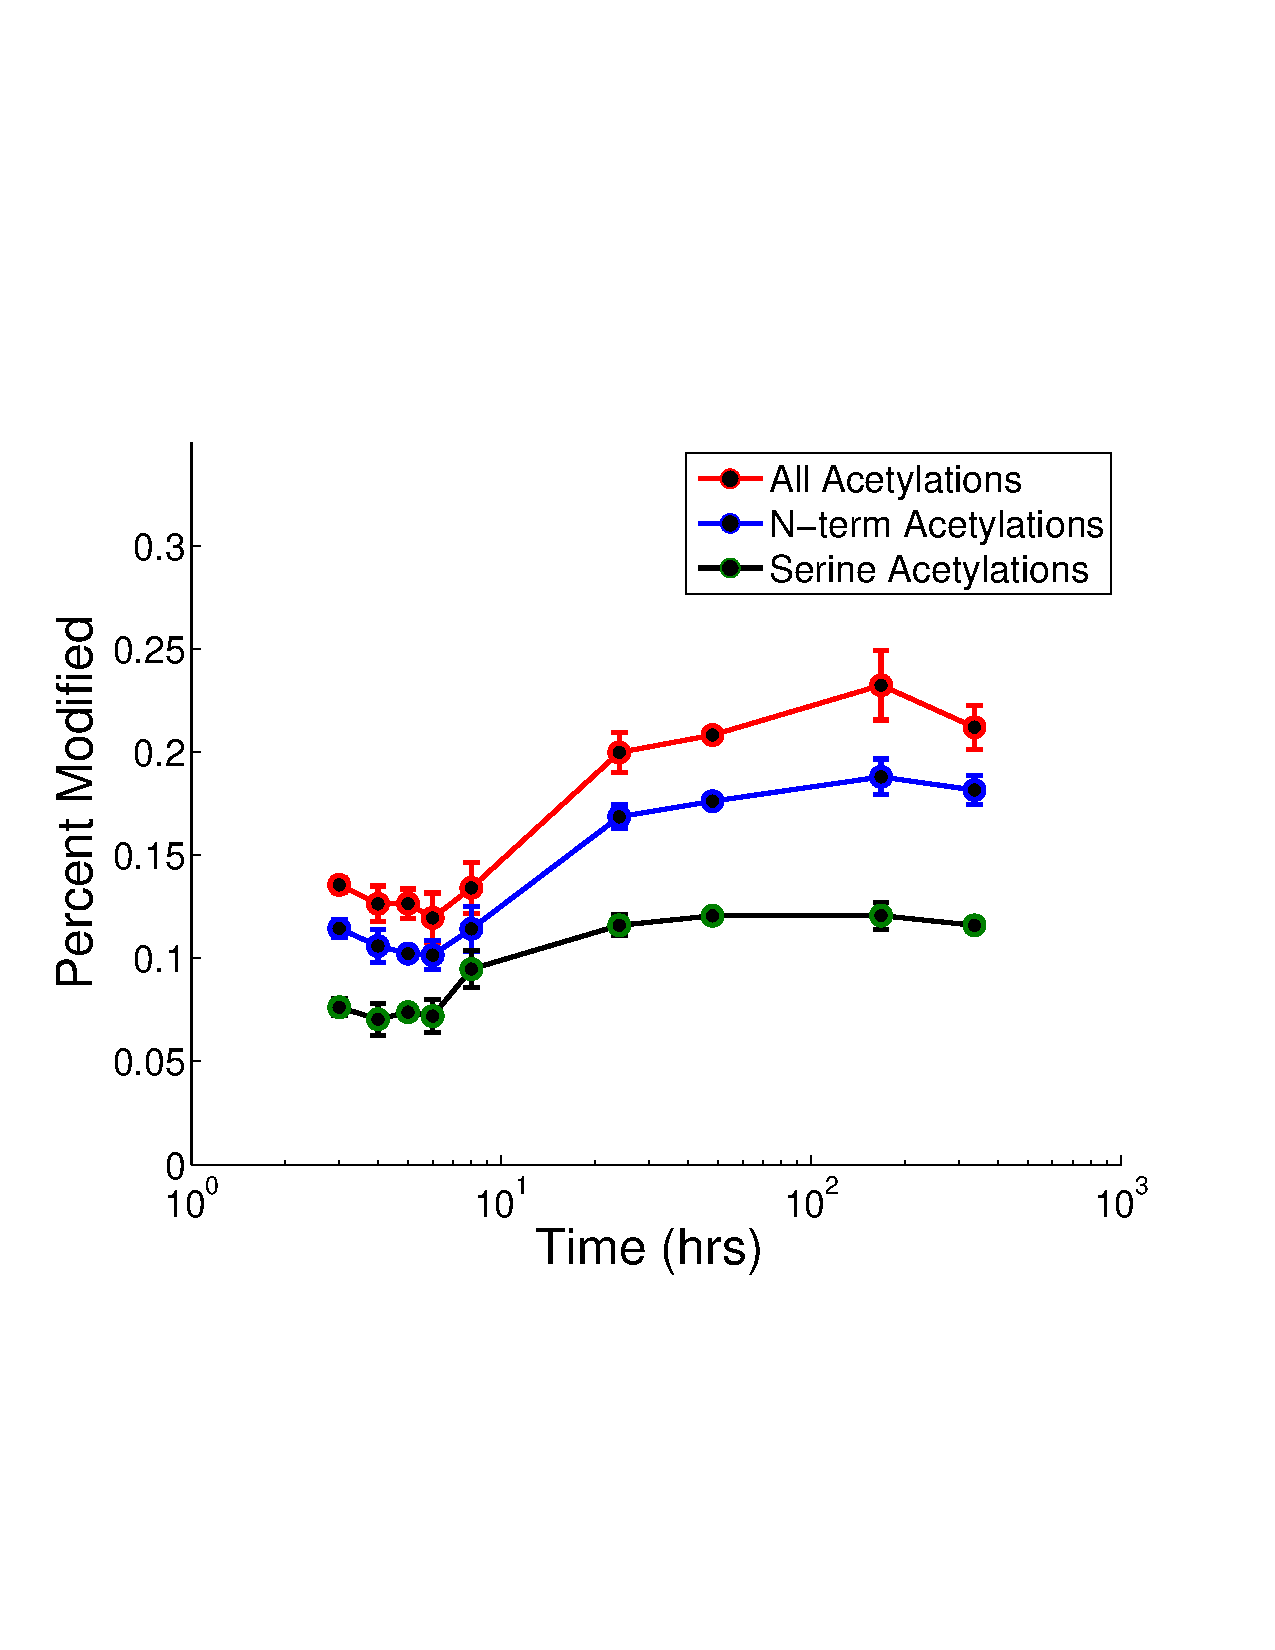
\includegraphics[width=5in]{Figures/Acetylation_AAs.pdf}}
\caption{\label{fig:Acet}\textbf{Protein n-term acetylations are dominant.} Total number of acetylations as well as the n-term/serine acetylations seem to go up over 2 weeks. \emph{E. coli} grown on glucose generally tend to accumulate acetate, perhaps this resulted in increase in acetylations.}\textbf{\emph{Is this percent of all PSMs, or all peptides?  What is the number value?}}
\end{figure}

\clearpage
\begin{figure}[p]
\centerline{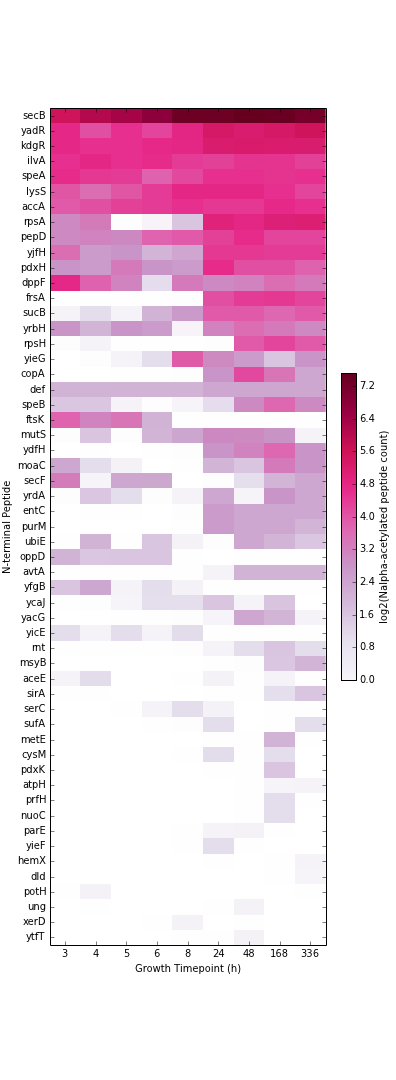
\includegraphics[width=5in]{Figures/AcetylatedProteins.png}}
\caption{\label{fig:Acet}\textbf{N-terminal acetylated peptides show differing patterns of NtAc across growth timepoints.} Counts for all peptides the protein's N-terminus and containing an Nt-acetylation (either a 42 or 43 Da mass shift) were summed across three biological replicates for each timepoint.  Color intensity shows log2-transformed, non-normalized NtAc peptide count for each timepoint. Proteins (rows) are sorted by mean abundance across all timepoints, with most abundant at the top.}
\end{figure}

\clearpage
\begin{figure}[p]
\centerline{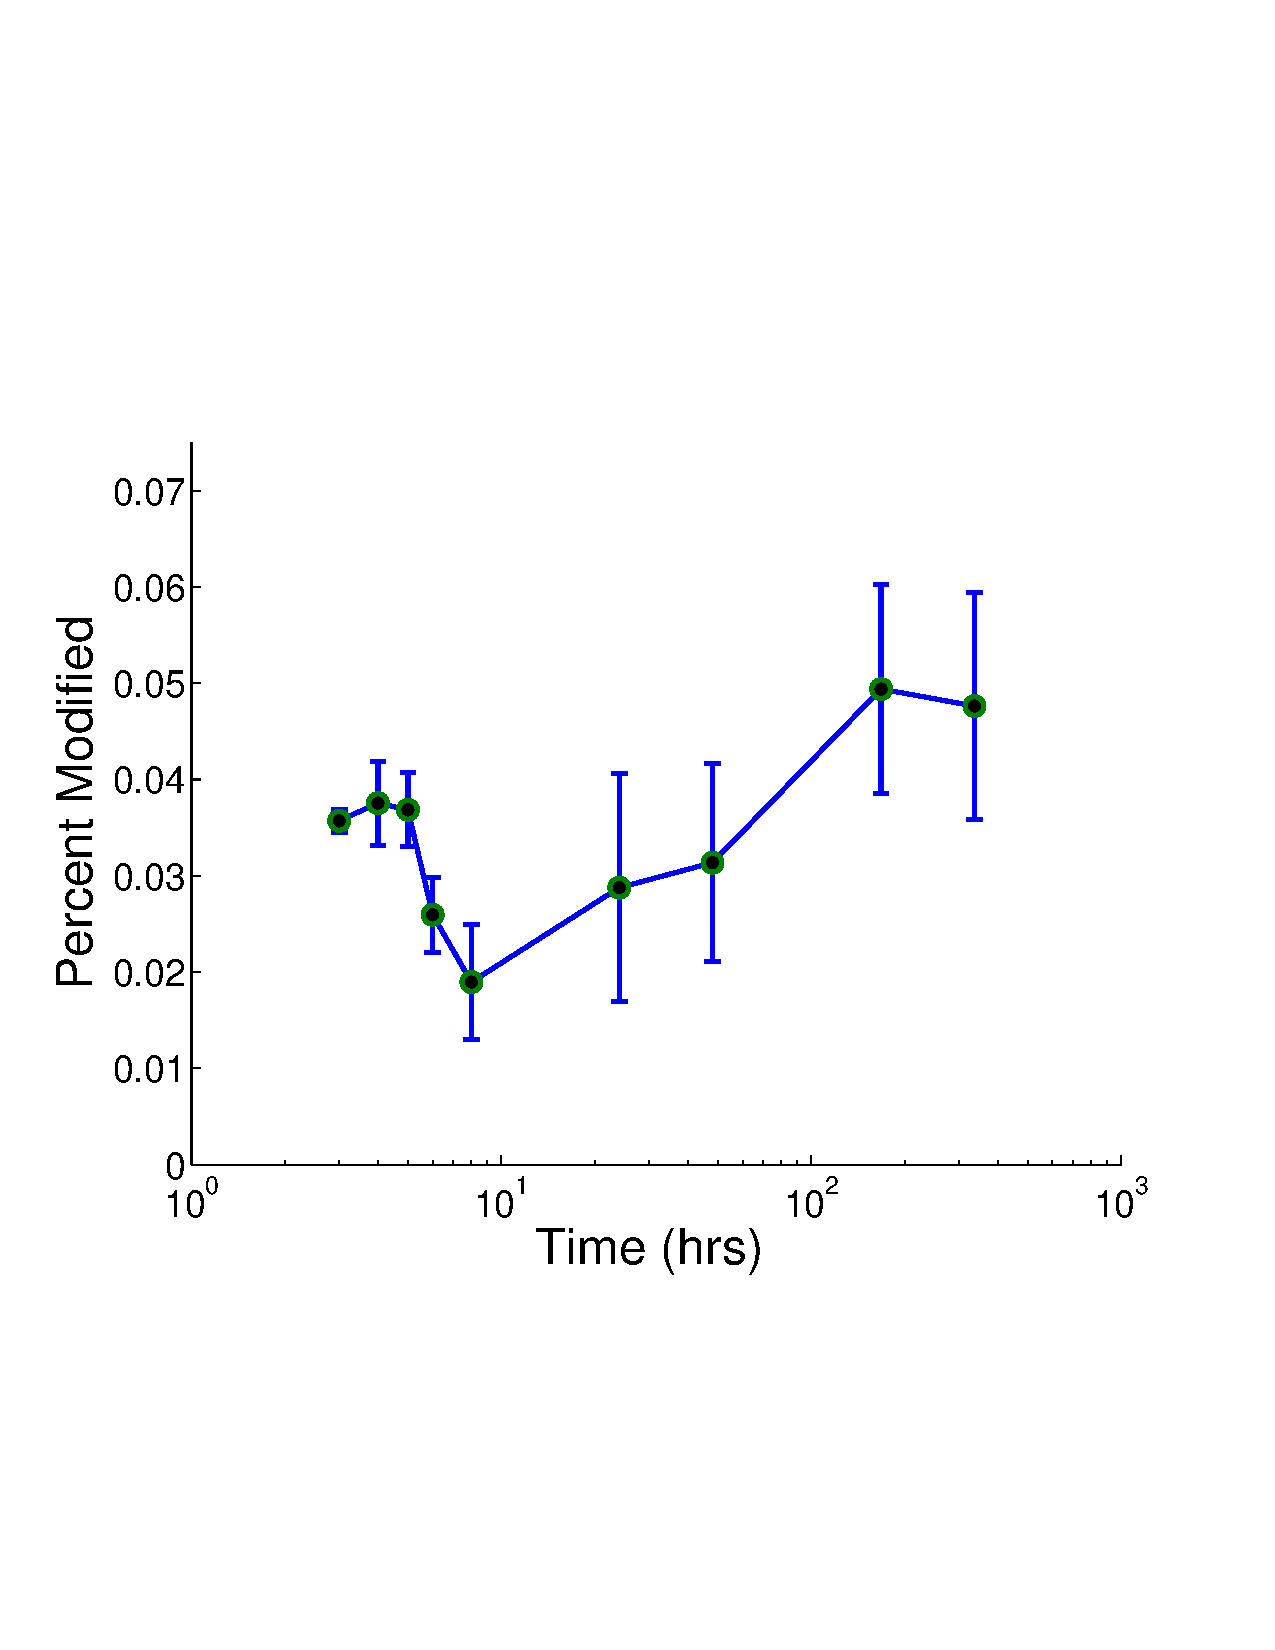
\includegraphics[width=5in]{Figures/Phosphorylations.pdf}}
\caption{\label{fig:Phos}\textbf{Phosphorylations are rare.} Phosphorylations seem to be low and tend to increase during last week of growth. 2 frequently phosphorylated proteins in MODa search output are phosphoglucomutase and elongation factor Tu.}
\end{figure}

\clearpage
\begin{figure}[p]
\centerline{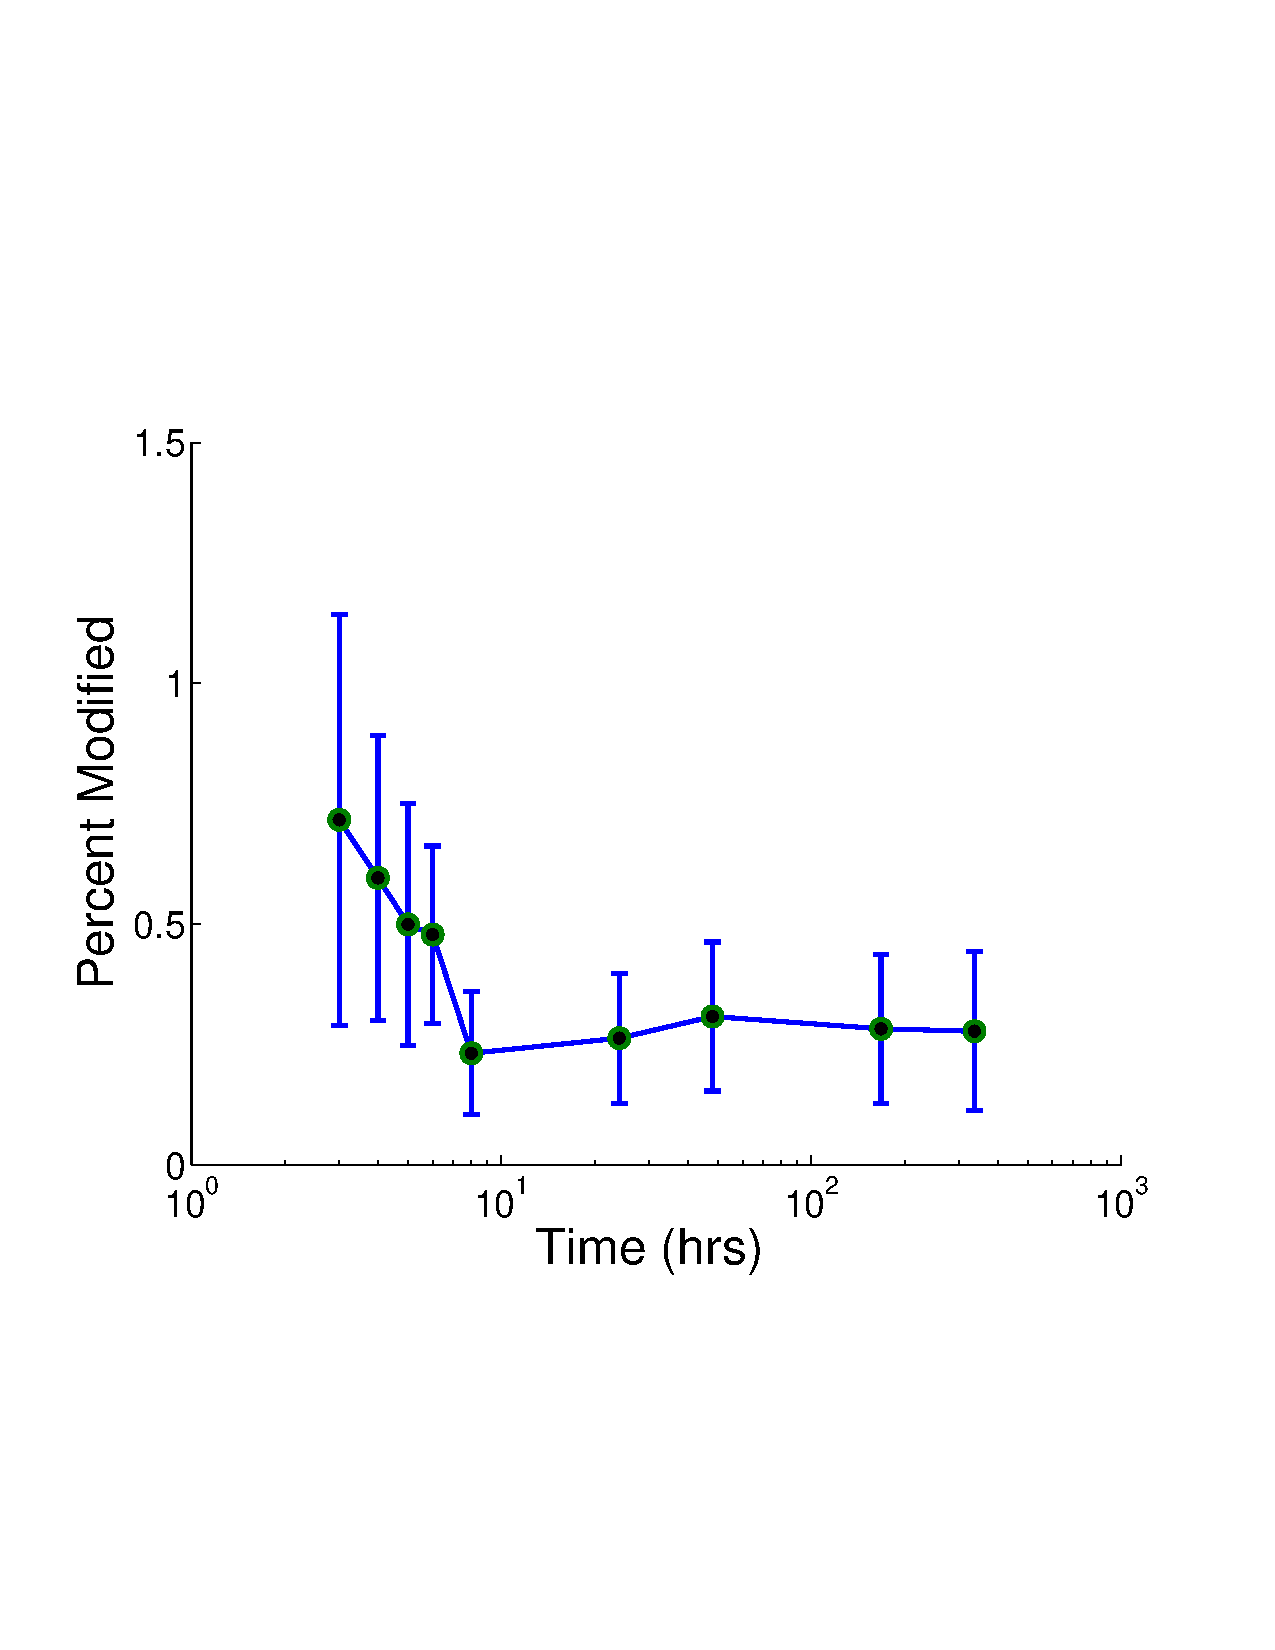
\includegraphics[width=5in]{Figures/MetGluTimeCourse.pdf}}
\caption{\label{fig:Phos}\textbf{Methionine to Glutamine subsitution.} .}
\end{figure}


\clearpage
\begin{figure}[p]
\centerline{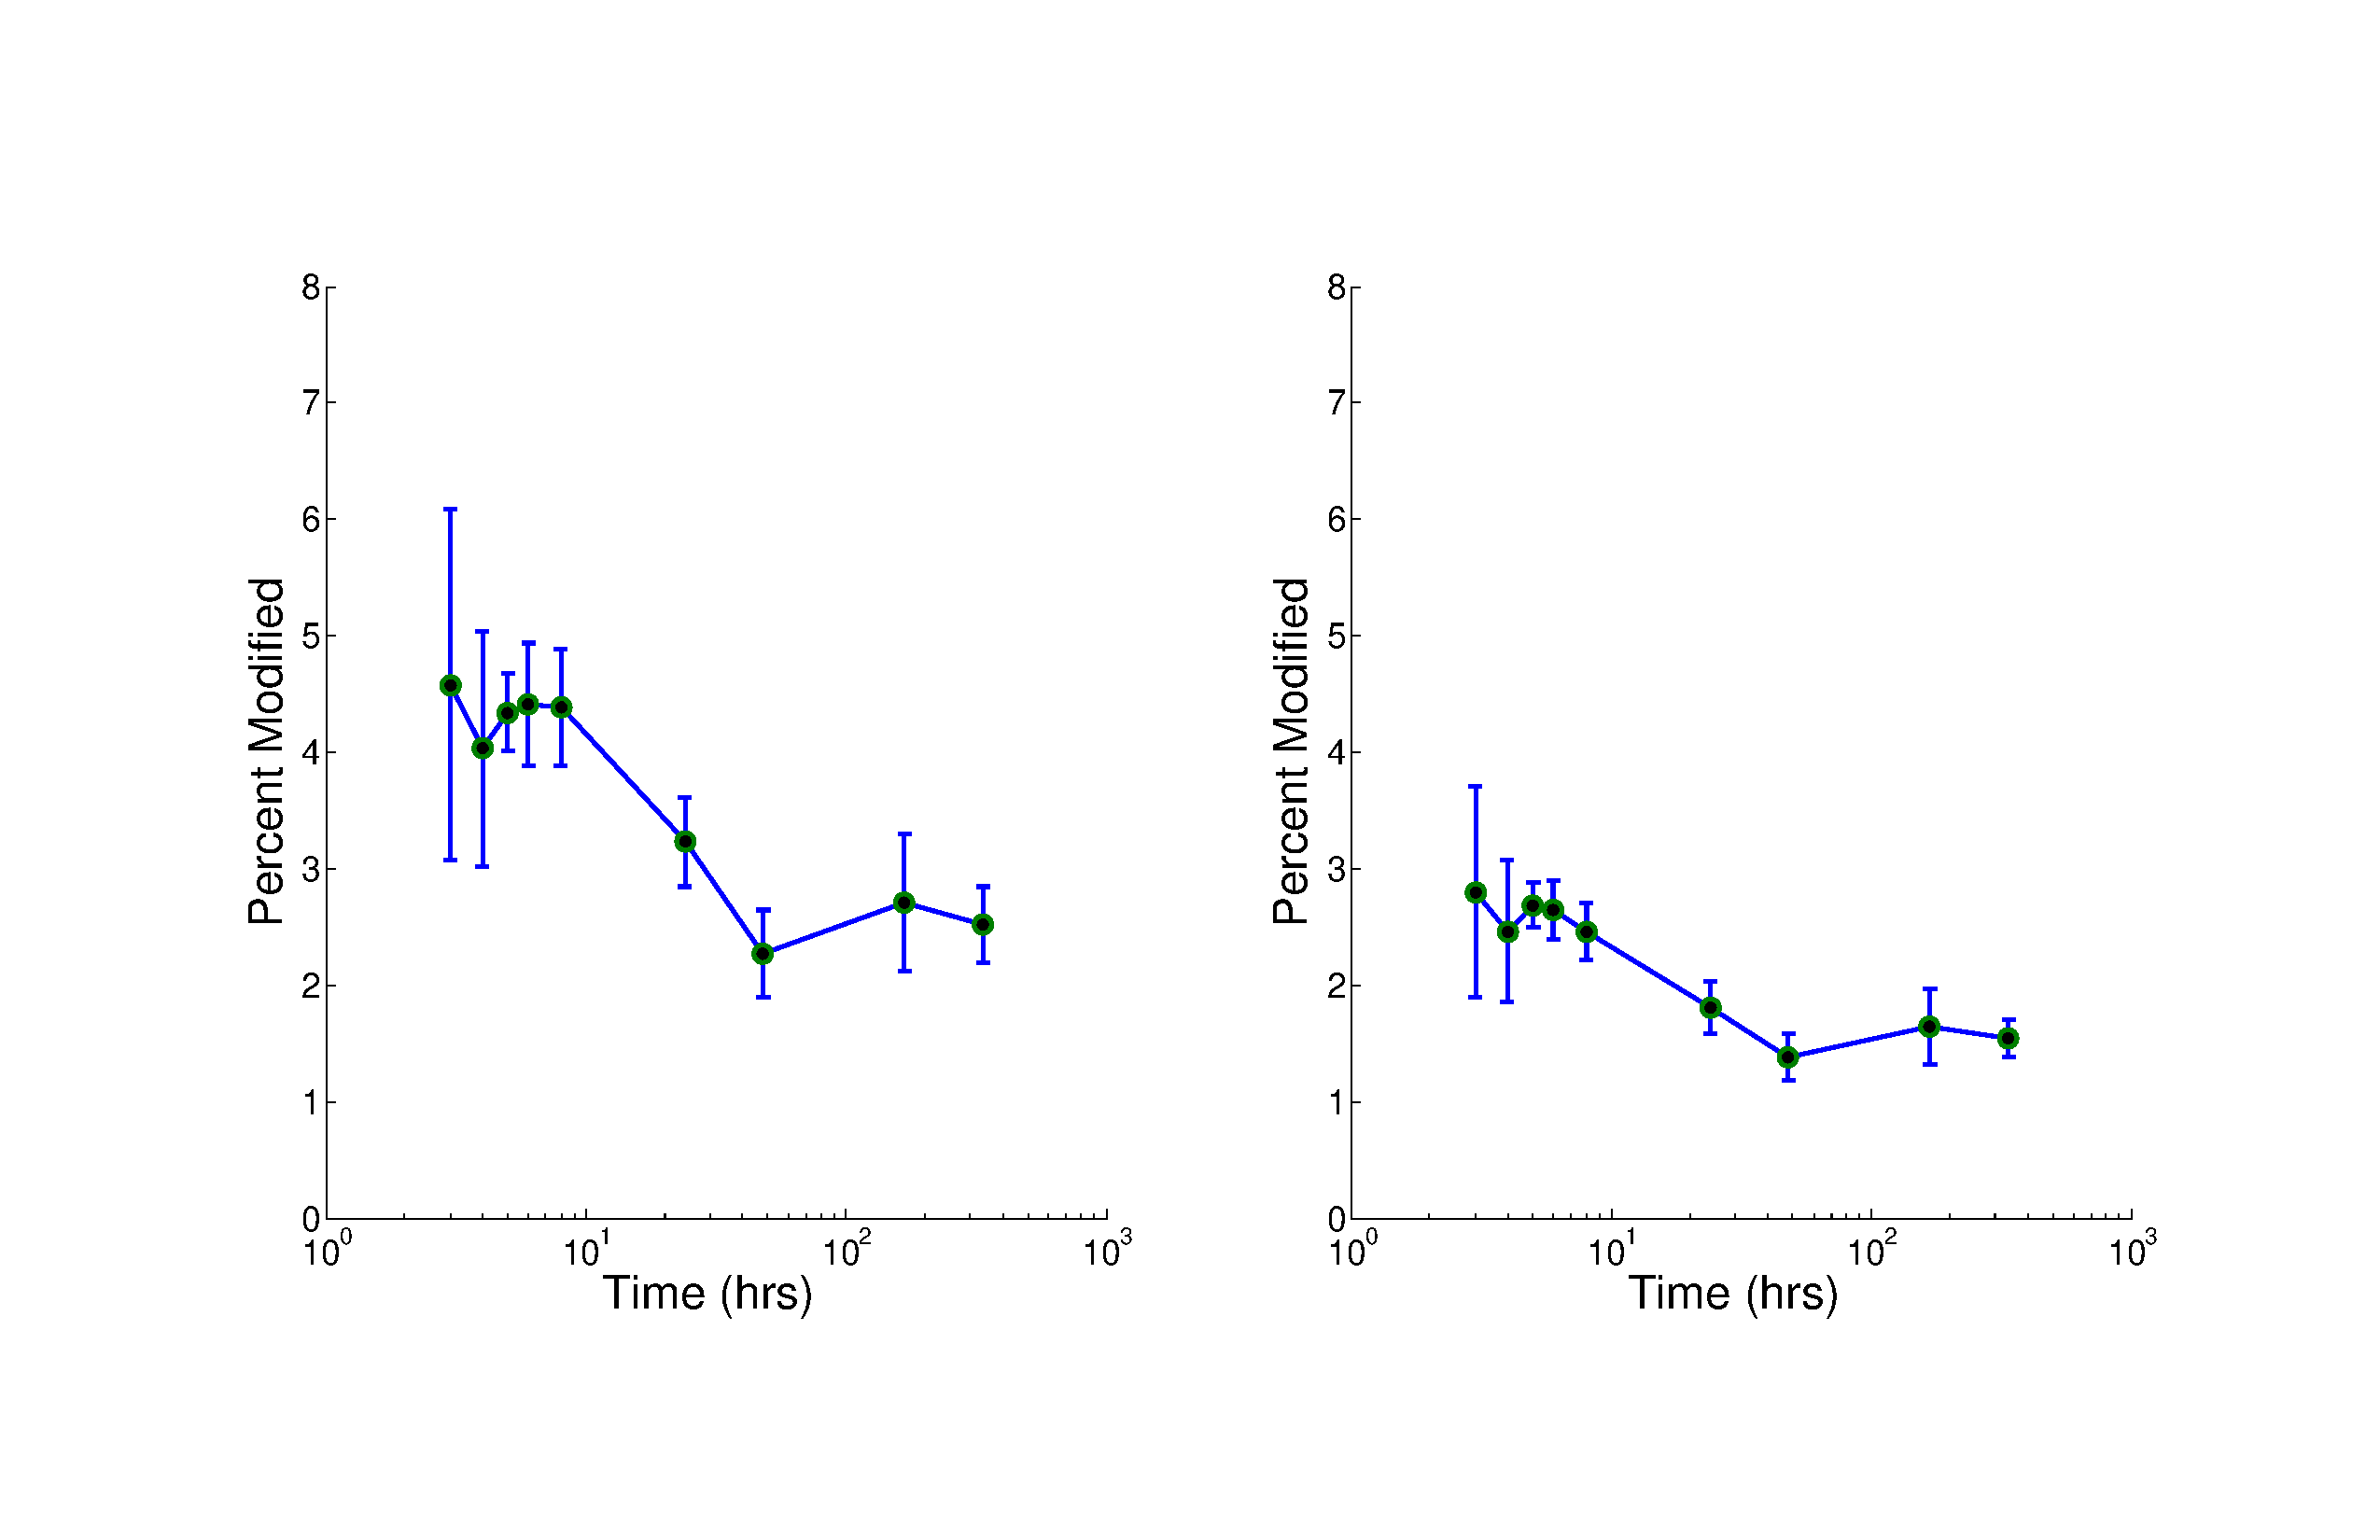
\includegraphics[width=8in]{Figures/Oxidations.pdf}}
\caption{\label{fig:Oxid}\textbf{Oxidations go down over 2 weeks.} (A) Total number of oxidations seem to go down from exponential to stationary phases. (B) The same trend follows for methionine oxidations too.}
\end{figure}

\clearpage
\begin{figure}[p]
\centerline{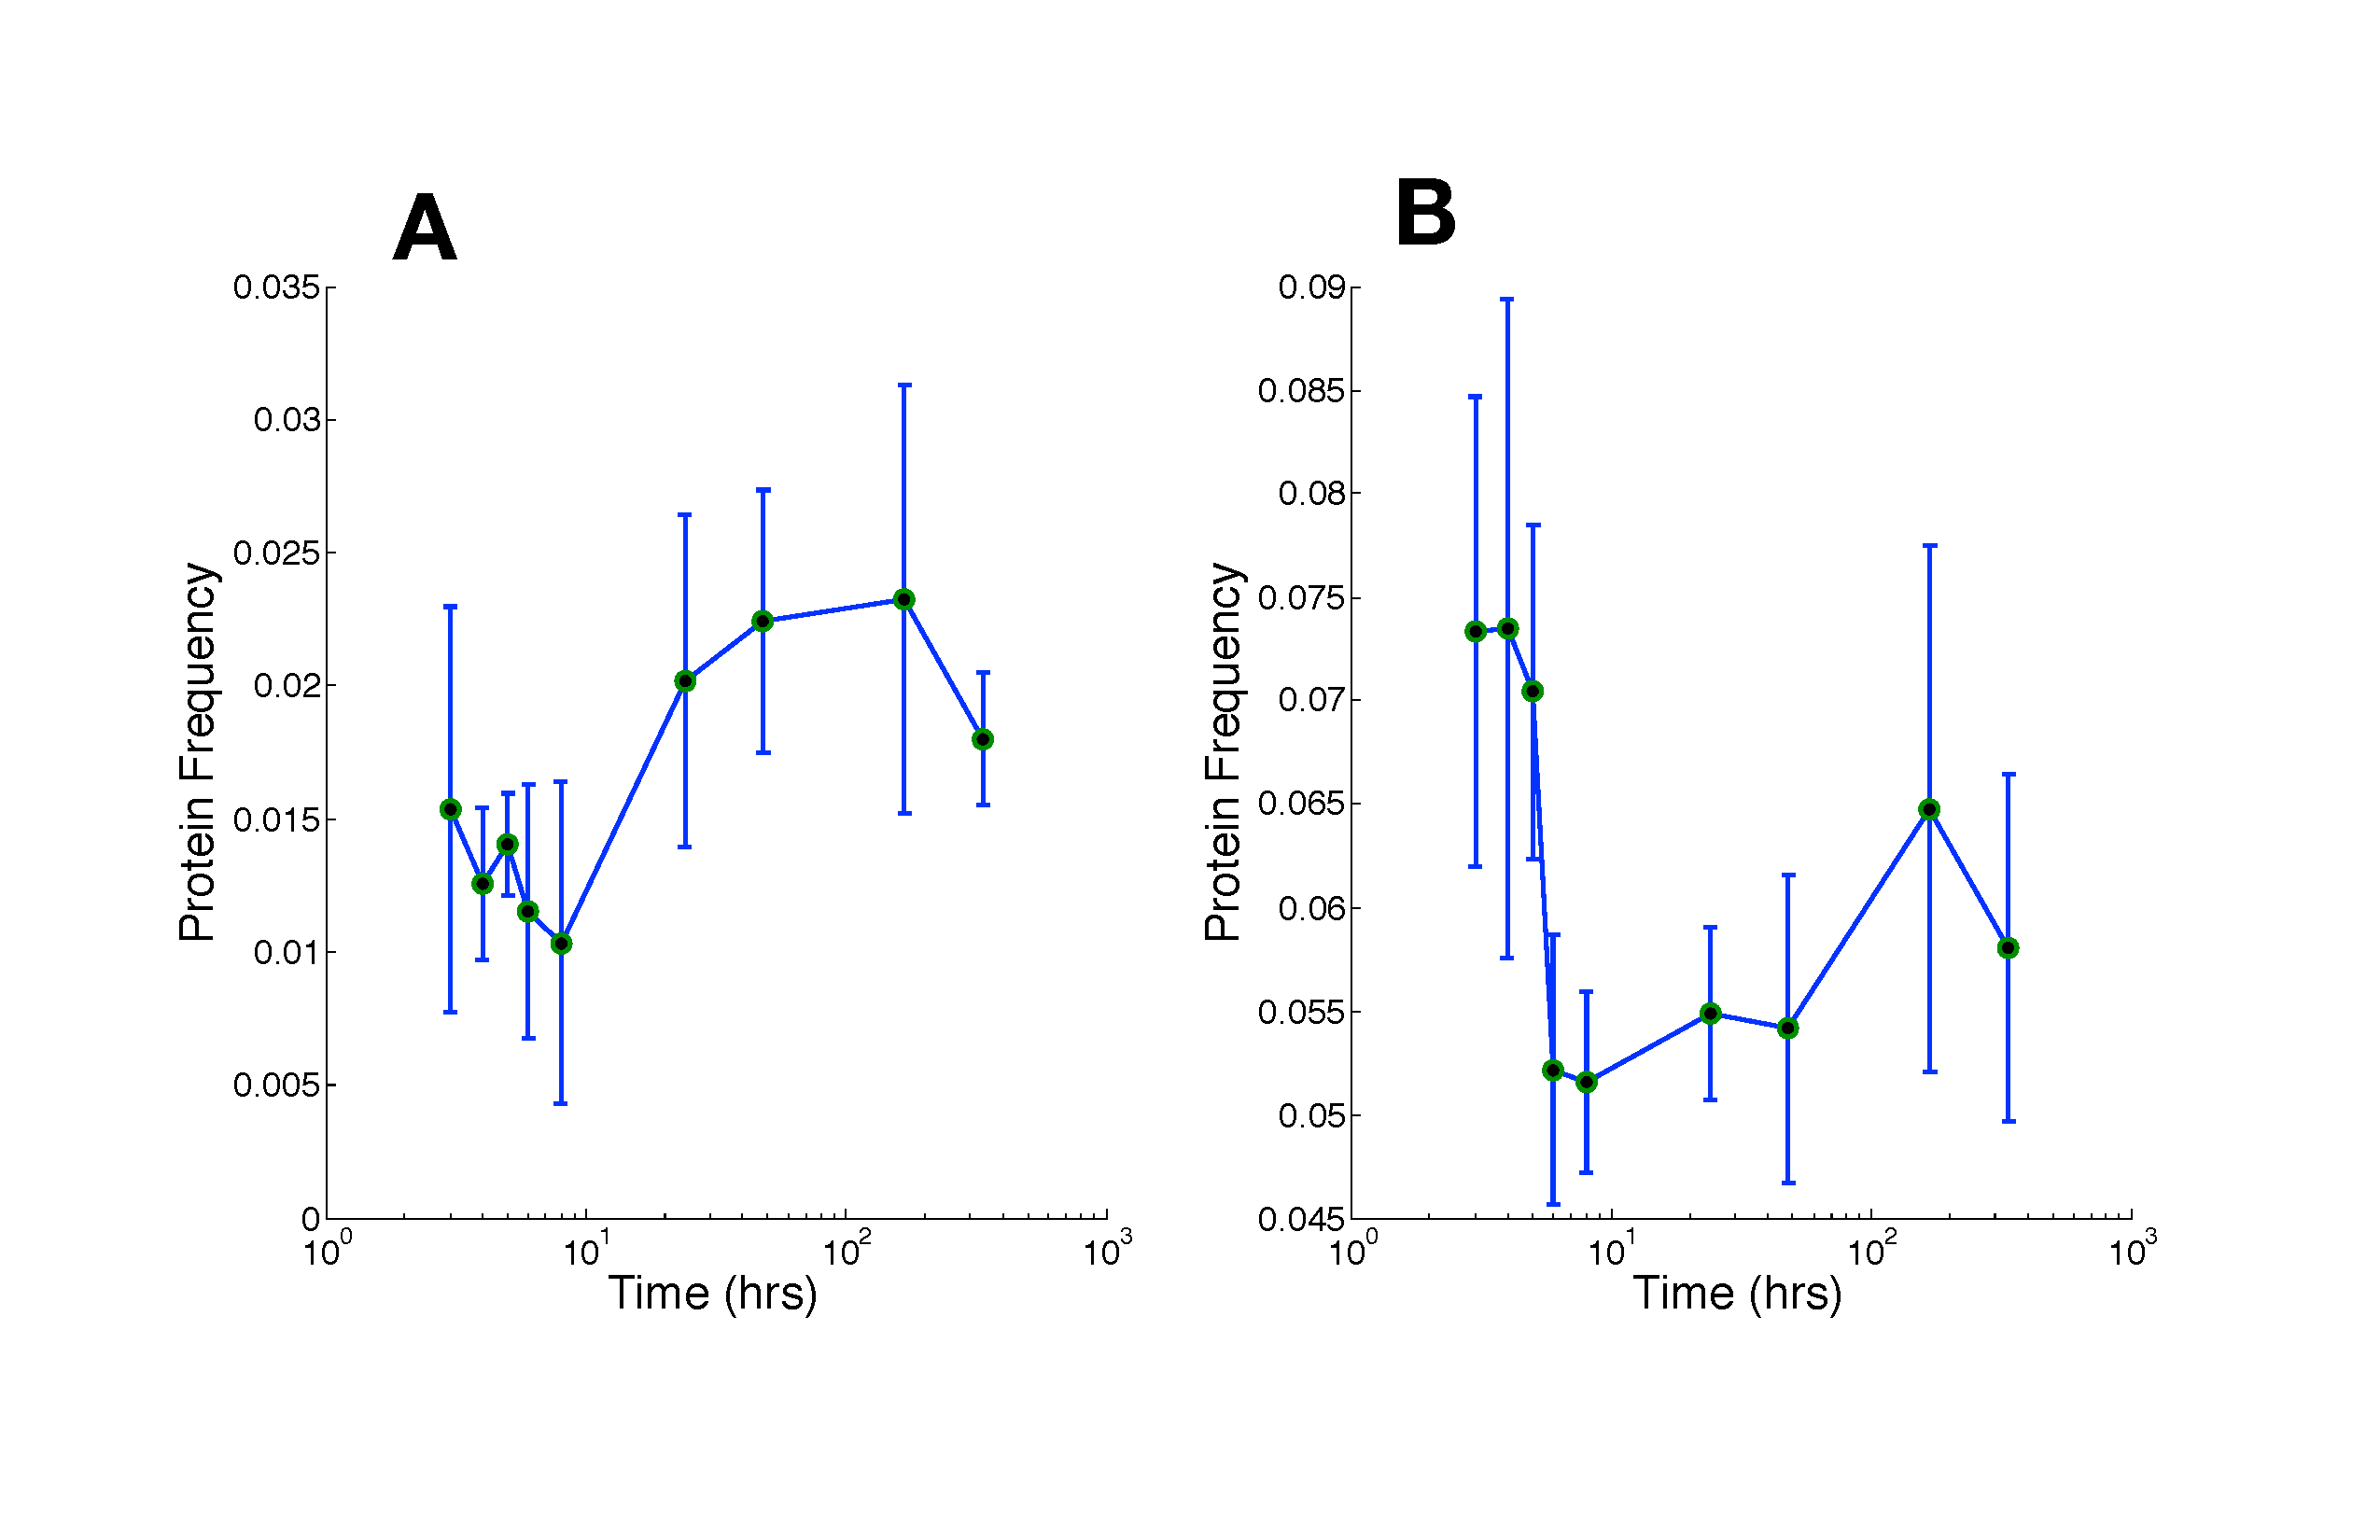
\includegraphics[width=8in]{Figures/Ecoli_MsrAB_MODa.pdf}}
\caption{\label{fig:MsrAB}\textbf{Relative protein abundances of methionine sulfoxide reductases MsrA and MsrB.} (A) Protein abundances of MsrA seems to increase going from exponential to long-stationary phase. One of the sites oxidized on MsrA is FQAA[M+16]LAADDDR. (B) MsrB also seems to increase going into the long-stationary phase, protecting \emph{E. coli} from oxidative damage.}
\end{figure}

\clearpage
\section*{Tables}
\begin{table}{!ht}
\caption{\label{tab:FrequentPSMs}
\textbf{This table lists the top 3 abundant hits at each one of the biological replicates and all the time points of the growth}}
\bigskip

\centerline{
\begin{tabular}{ccc}
\textbf{Frequency} & \textbf{Peptide} & \textbf{Biological Replicate} \\
\hline
28&M.S+42EQNNTEMTFQIQR.I&10\\
25&R.I+2TTSHYDVGGAAIDNHGQPLPPATVEGCEQADAVLFGSVGGPK.W&10\\
13&K.TPGHPEVGYTAGVETTTGP+2LGQGIANAVGMAIAEK.T&10\\
71&K.EGVITVEDGTG+23LQDELDVVEGMQFDR.G&11\\
39&M.S+42EQNNTEMTFQIQR.I&11\\
28&R.KMDAFIQYGIVAGVQ+2AMQDSGLEITEENATR.I&11\\
57&K.EGVITVEDGTG+23LQDELDVVEGMQFDR.G&12\\
34&M.S+42EQNNTEMTFQIQR.I&12\\
23&K.EGVITVEDGTGLQDE+23LDVVEGMQFDR.G&12\\
67&K.EGVITVEDGTG+23LQDELDVVEGMQFDR.G&13\\
32&M.S+42EQNNTEMTFQIQR.I&13\\
25&K.EGVITVEDGT+23GLQDELDVVEGMQFDR.G&13\\
37&K.EGVITVEDGTG+23LQDELDVVEGMQFDR.G&14\\
33&M.S+42EQNNTEMTFQIQR.I&14\\
28&M.S+43EQNNTEMTFQIQR.I&14\\
55&K.EGVITVEDGTG+23LQDELDVVEGMQFDR.G&15\\
41&K.AEIFSLFAENN+23MELTDSTIVTPGLR.F&15\\
29&M.S+42EQNNTEMTFQIQR.I&15\\
15&M.S+42EQNNTEMTFQIQR.I&16\\
13&K.LVSW+32YDNETGYSNK.V&16\\
8&M.S+42LNFLDFEQPIAELEAK.I&16\\
22&M.S+42EQNNTEMTFQIQR.I&17\\
12&K.EGVITVEDGT+23GLQDELDVVEGMQFDR.G&17\\
11&K.EGVITVEDGTG+23LQDELDVVEGMQFDR.G&17\\
26&M.S+42EQNNTEMTFQIQR.I&18\\
10&R.I+2TTSHYDVGGAAIDNHGQPLPPATVEGCEQADAVLFGSVGGPK.W&18\\
10&M.A+42DSQPLSGTPEGAEYLR.A&18\\
26&M.S+42EQNNTEMTFQIQR.I&19\\
15&K.NMITGAAQMDGAI+39LVVAATDGPMPQTR.E&19\\
14&K.DGAVEAEDRVTI+2DFTGSVDGEEFEGGK.A&19\\
53&M.S+42EQNNTEMTFQIQR.I&20\\
32&K.NMITGAAQMDGAI+39LVVAATDGPMPQTR.E&20\\
20&K.EISPYSIVGLSATW+32DVTK.N&20\\
48&M.S+42EQNNTEMTFQIQR.I&21\\
29&K.EGVITVEDGTGLQDE+23LDVVEGMQFDR.G&21\\
17&K.EGVITVEDGTG+24LQDELDVVEGMQFDR.G&21\\
47&M.S+42EQNNTEMTFQIQR.I&22\\
17&K.DGAVEAEDRVTI+2DFTGSVDGEEFEGGK.A&22\\
14&K.M+32MTMLDPANAER.Y&22\\
30&K.M+32MTMLDPANAER.Y&23\\
25&M.S+42EQNNTEMTFQIQR.I&23\\
20&K.EGVITVEDGTGLQDE+23LDVVEGMQFDR.G&23\\
27&K.EGVITVEDGTGLQDE+23LDVVEGMQFDR.G&24\\
25&M.S+42EQNNTEMTFQIQR.I&24\\
23&K.EGVITVEDGTG+23LQDELDVVEGMQFDR.G&24\\
21&K.W+32FNTNYHYMVPEFVK.G&25\\
15&K.LVSW+32YDNETGYSNK.V&25\\
12&K.M+42ETTKPSFQDVLEFVR.L&25\\
22&K.W+32FNTNYHYMVPEFVK.G&26\\
21&M.S+42EQNNTEMTFQIQR.I&26\\
16&R.G+57ITINTSHVEYDTPTR.H&26\\
21&M.S+42EQNNTEMTFQIQR.I&27\\
20&K.W+32FNTNYHYMVPEFVK.G&27\\
15&R.EAEGSHIMLGAQNVDL+2NLSGAFTGETSAAMLK.D&27\\
30&M.S+42EQNNTEMTFQIQR.I&28\\
24&R.KMDAFIQYGIVAGVQ+2AMQDSGLEITEENATR.I&28\\
18&R.KMDAFIQYGIVAGV+2QAMQDSGLEITEENATR.I&28\\
35&M.S+42EQNNTEMTFQIQR.I&29\\
19&K.APSLLQLSPDW+32TSNSCR.G&29\\
13&K.AMLQDIA+2TLTGGTVISEEIGMELEK.A&29\\
39&M.S+42EQNNTEMTFQIQR.I&30\\
30&K.EGVITVEDGTGLQDE+23LDVVEGMQFDR.G&30\\
18&K.W+4QTHLINPHIILSK.E&30\\
46&M.S+42EQNNTEMTFQIQR.I&31\\
36&K.EGVITVEDGTGLQDE+23LDVVEGMQFDR.G&31\\
22&K.EGVITVEDGTG+23LQDELDVVEGMQFDR.G&31\\
34&M.S+42EQNNTEMTFQIQR.I&32\\
19&K.EGVITVEDGTGLQDE+23LDVVEGMQFDR.G&32\\
19&K.EGVITVEDGTG+23LQDELDVVEGMQFDR.G&32\\
30&R.KMDAFIQYGIVAGVQ+2AMQDSGLEITEENATR.I&33\\
27&M.S+42EQNNTEMTFQIQR.I&33\\
17&R.KMDAFIQYGIVAGV+2QAMQDSGLEITEENATR.I&33\\
13&M.S+42EQNNTEMTFQIQR.I&7\\
11&R.NVTVM+32AMDSVPR.I&7\\
10&K.N+62VFAELDVSWDK.N&7\\
17&M.S+42EQNNTEMTFQIQR.I&8\\
17&K.NMITGAAQM+23DGAILVVAATDGPMPQTR.E&8\\
12&K.EFWNVVNW+32DEAAAR.F&8\\
18&M.S+42EQNNTEMTFQIQR.I&9\\
11&K.NMITGAAQM+23DGAILVVAATDGPMPQTR.E&9\\
8&M.A+42DSQPLSGTPEGAEYLR.A&9\\
\hline
\end{tabular}
}
\end{table}

\bigskip
\section*{Supplementary Figures}
\clearpage
\centerline{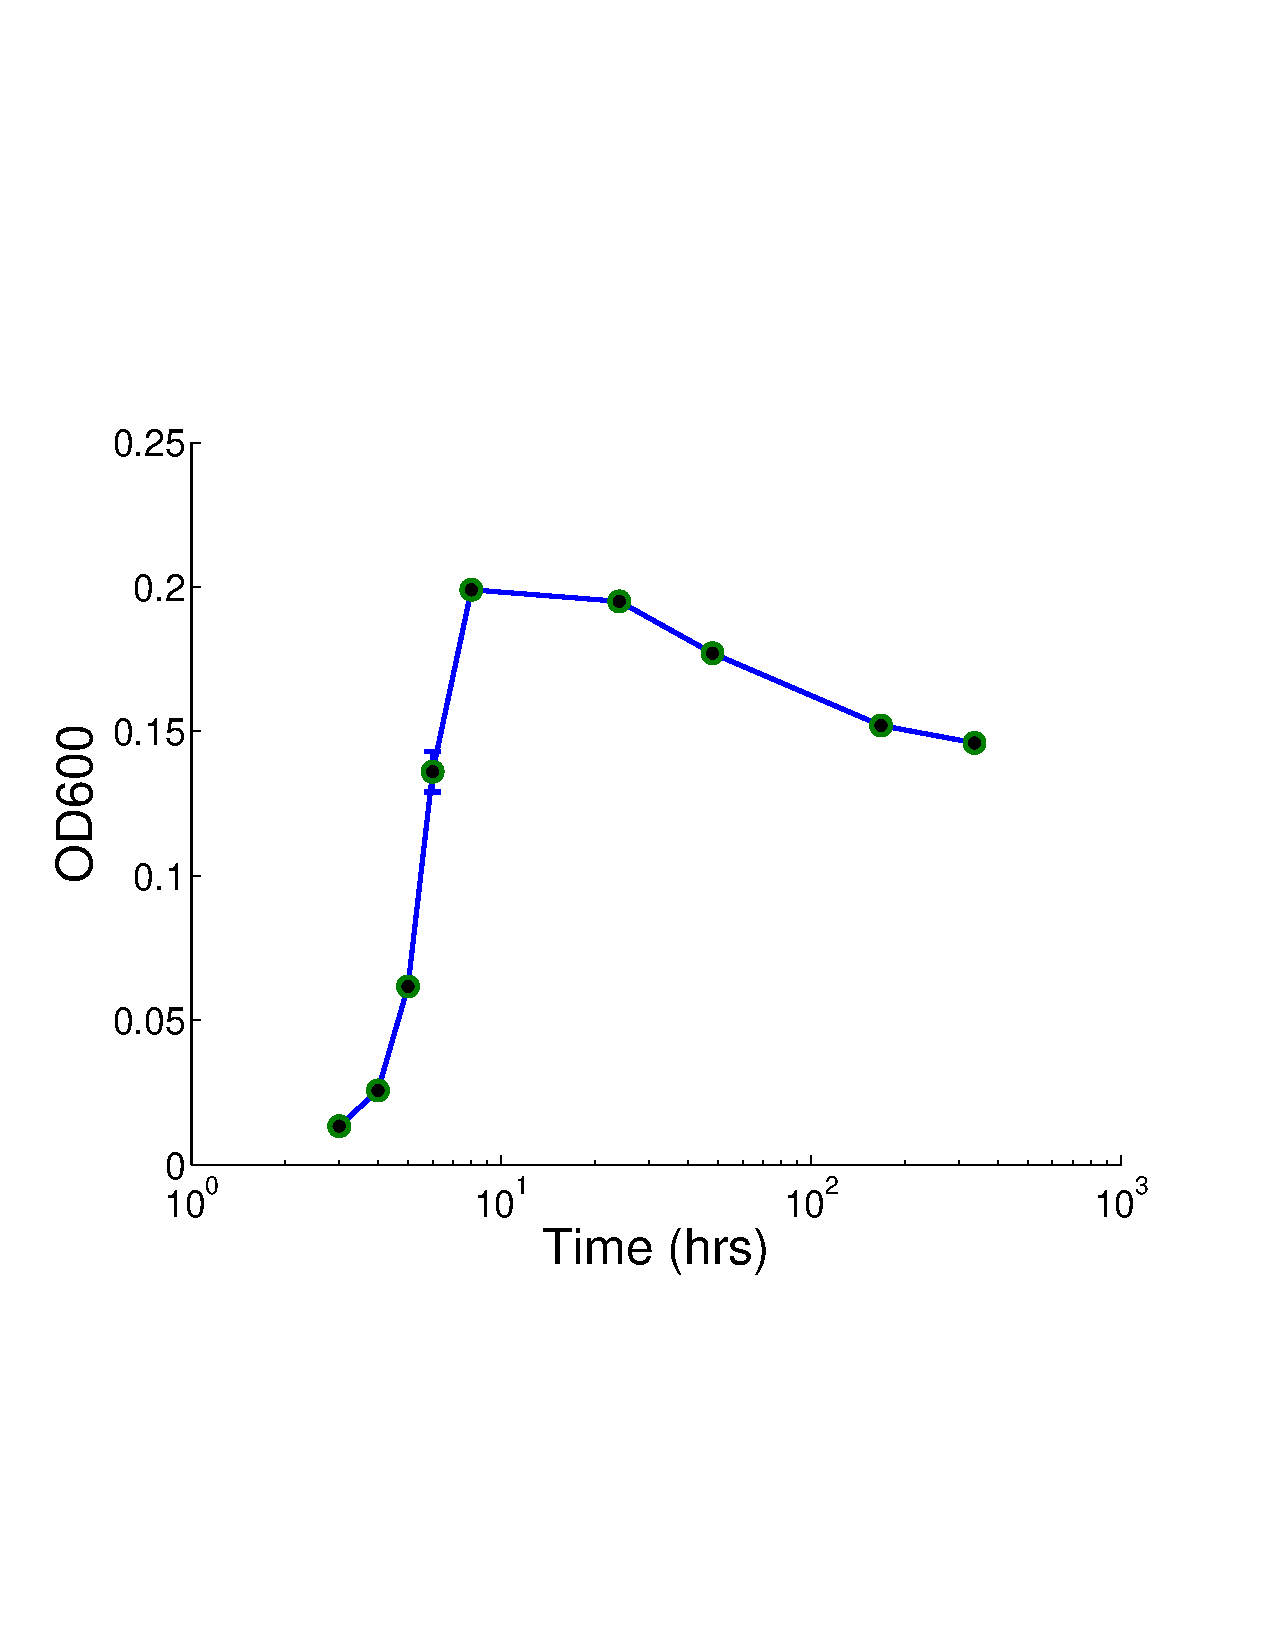
\includegraphics[width=5in]{Figures/GrowthCurve.pdf}}
\customlabel{fig:GrowthCurveFig}{S1}
\textbf{Figure S1: OD600 curve .}  Growth curve (OD600) of REL606 under glucose starvation conditions.

\clearpage
\centerline{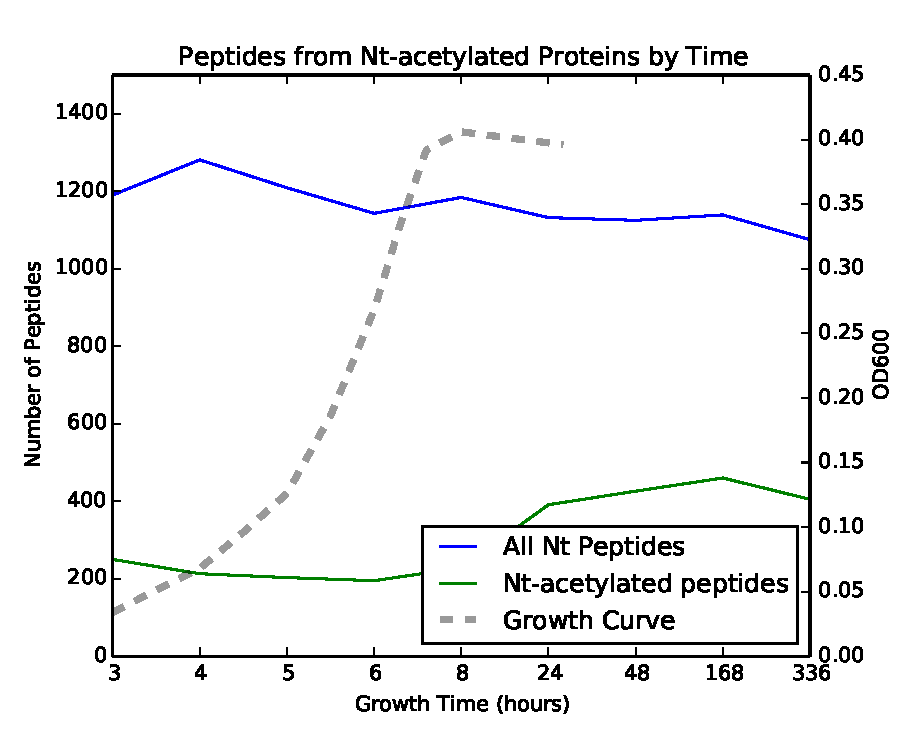
\includegraphics[width=5in]{Figures/AcetylatedPeptides.pdf}}
\customlabel{fig:ActPeptidesFig}{S2}
\textbf{Figure S2: N-terminal Nalpha Acetylated Peptide Occurance across Growth Timepoints.} Blue line represents total count of N-terminal peptides with any (or no) modification originating from parent proteins with at least one Nt-acetylated peptide in the dataset.  Green line represents total count of Nt-acetylated peptides from these proteins.  Both counts are the sum of three biological replicates for each timepoint. Dashed line (right axis) shows OD600 values for an example culture grown under identical glucose-starvation conditions.

\clearpage
\centerline{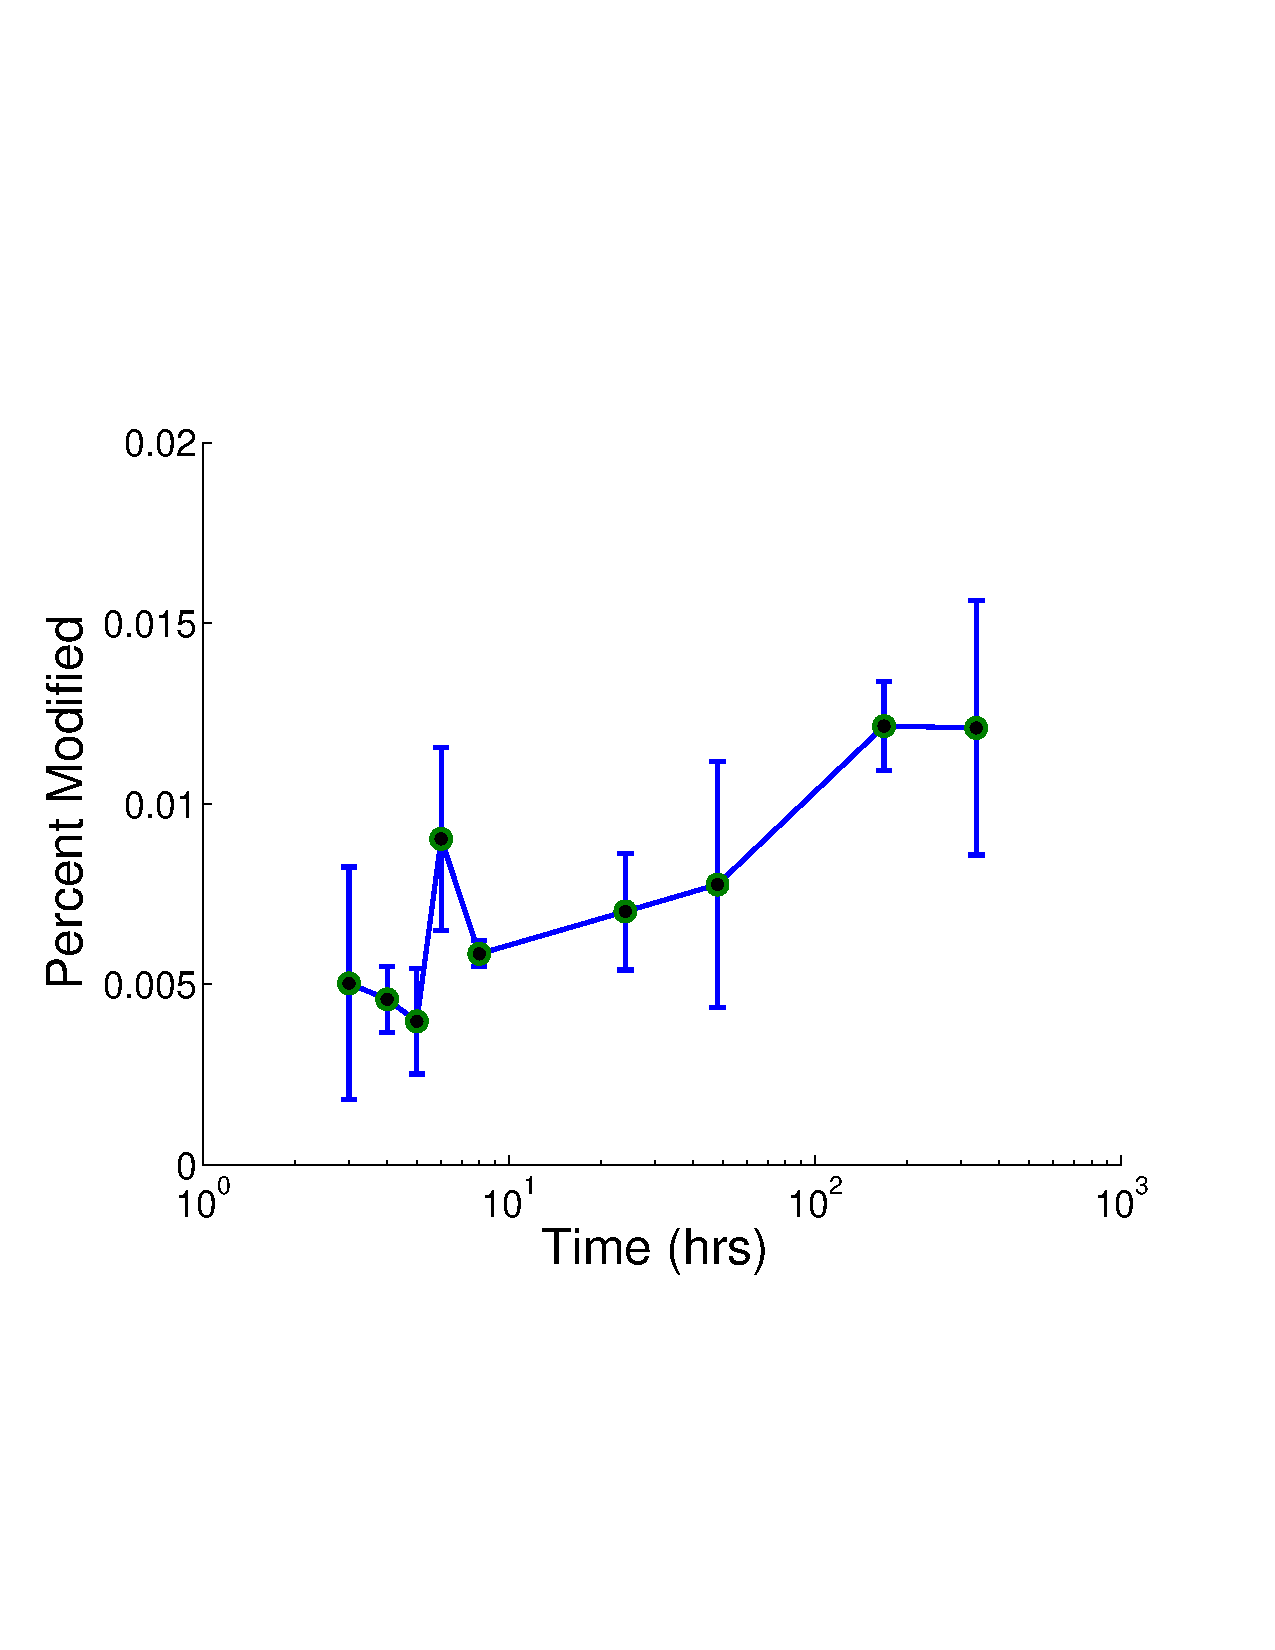
\includegraphics[width=5in]{Figures/Carboxylations.pdf}}
\customlabel{fig:CarboxylationFig}{S3}
\textbf{Figure S3: E. coli Carboxylations .} Carboxylations seem to go up.

\clearpage
\centerline{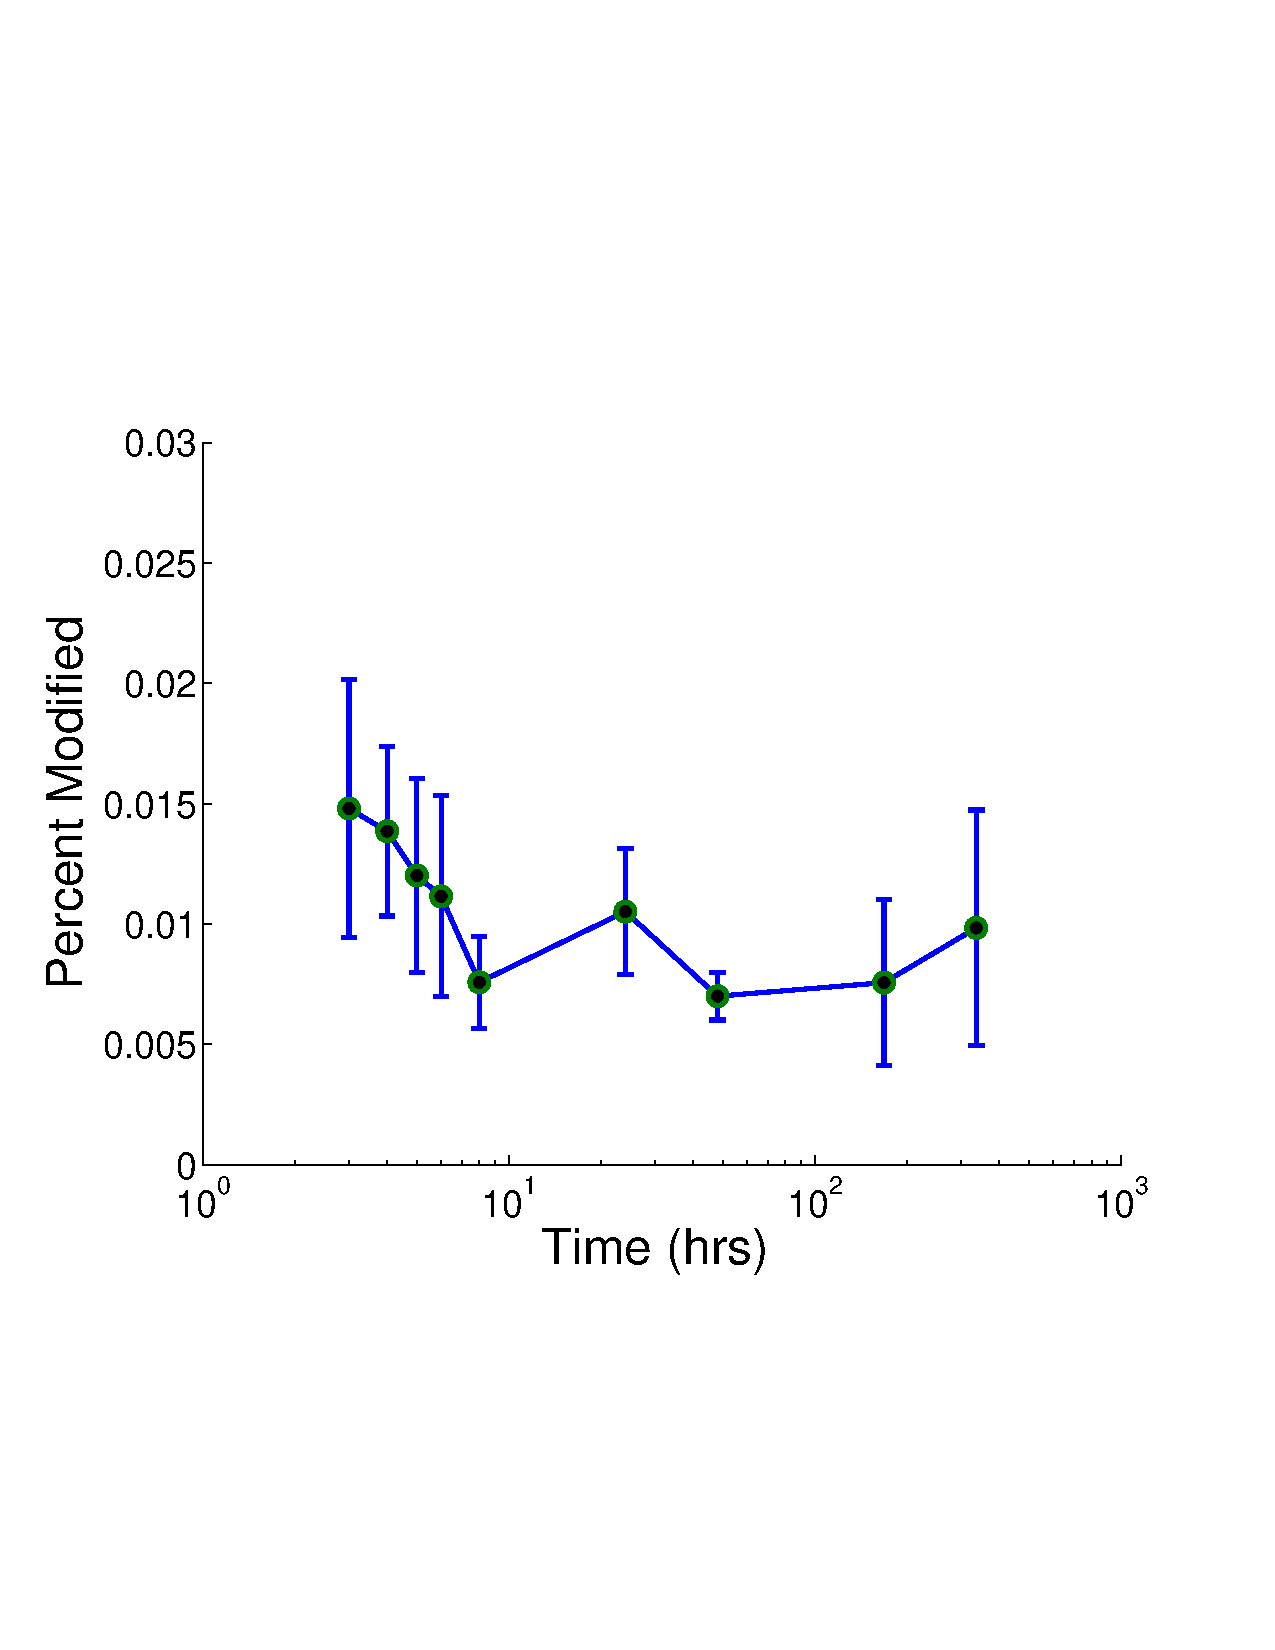
\includegraphics[width=5in]{Figures/Nitrosylations.pdf}}
\customlabel{fig:NitrosylationFig}{S4}
\textbf{Figure S4: E. coli Nitrosylations.} Nitrosylations seem not to change much during the entire growth period.

\clearpage
\centerline{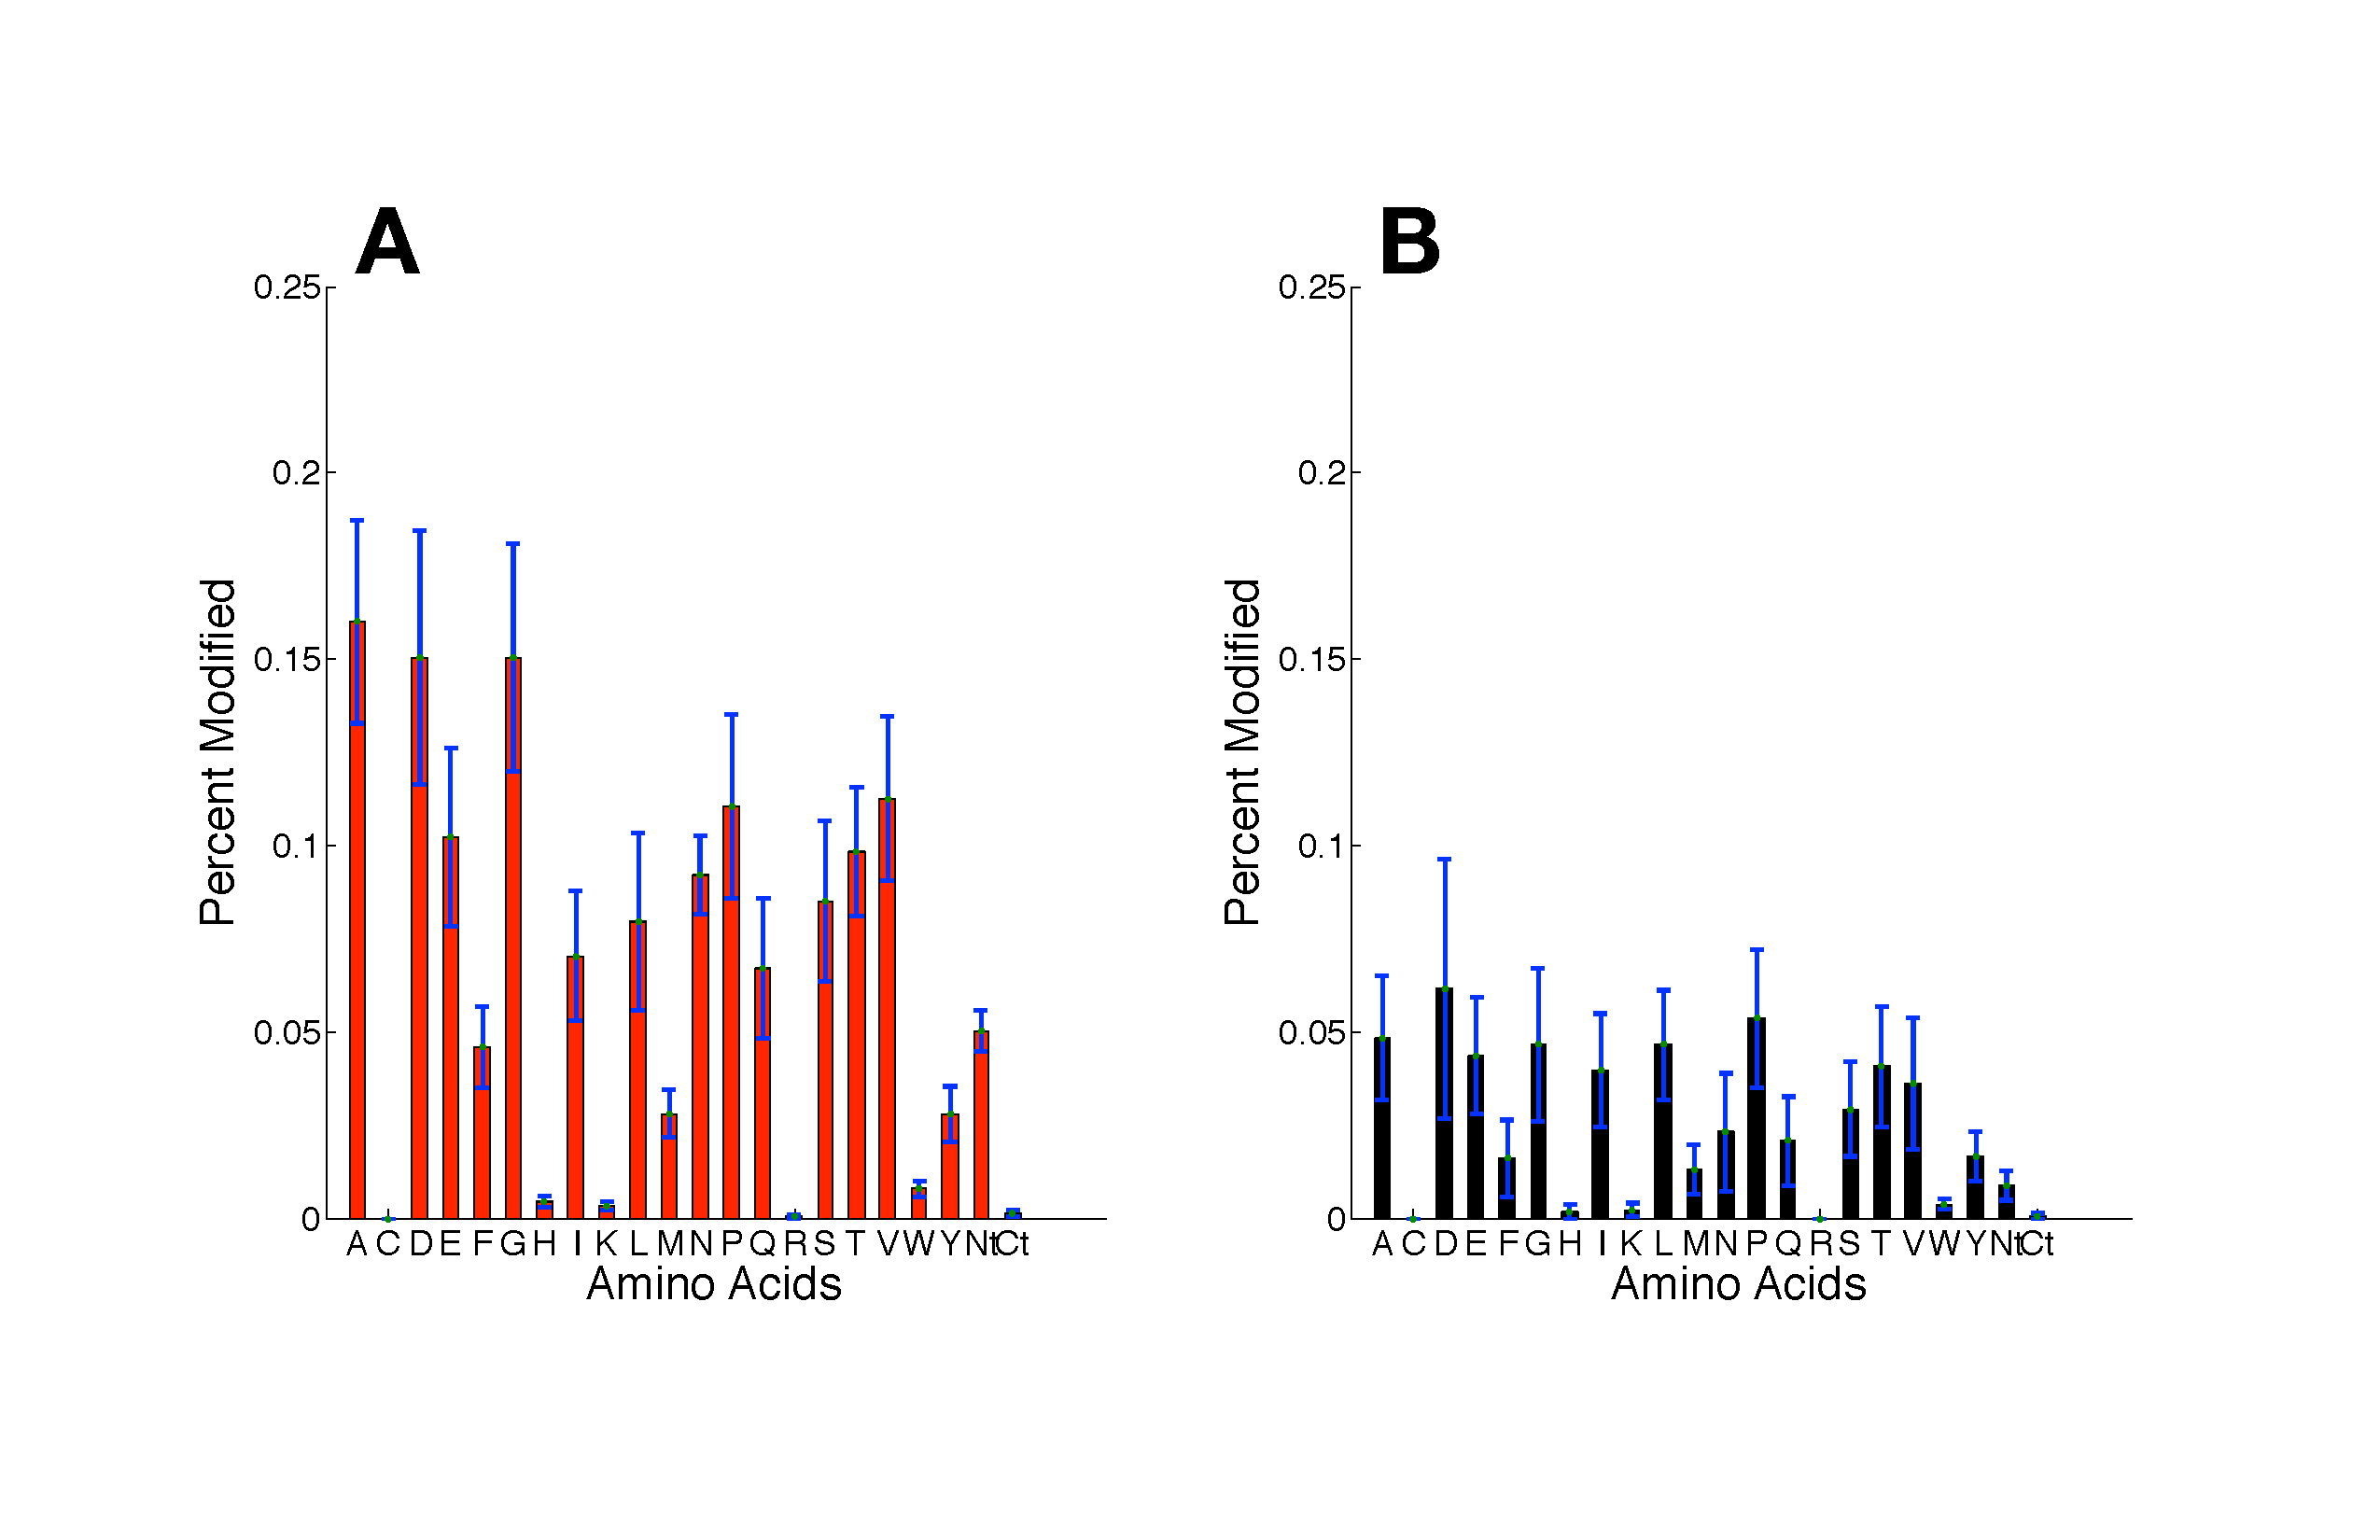
\includegraphics[width=8in]{Figures/NaKAdducts.pdf}}
\customlabel{fig:NaKAdductFig}{S5}
\textbf{Figure S5: Na and K adducts.} (A) Na and (B) K adducts seem to happen on all amino acids except histidine, lysine and arginine. H, K and R are amino acids that are basic and carry some (+) charge at physiological pH. Here Nt and Ct represent n-termins and c-terminus of the peptide.

\clearpage
\centerline{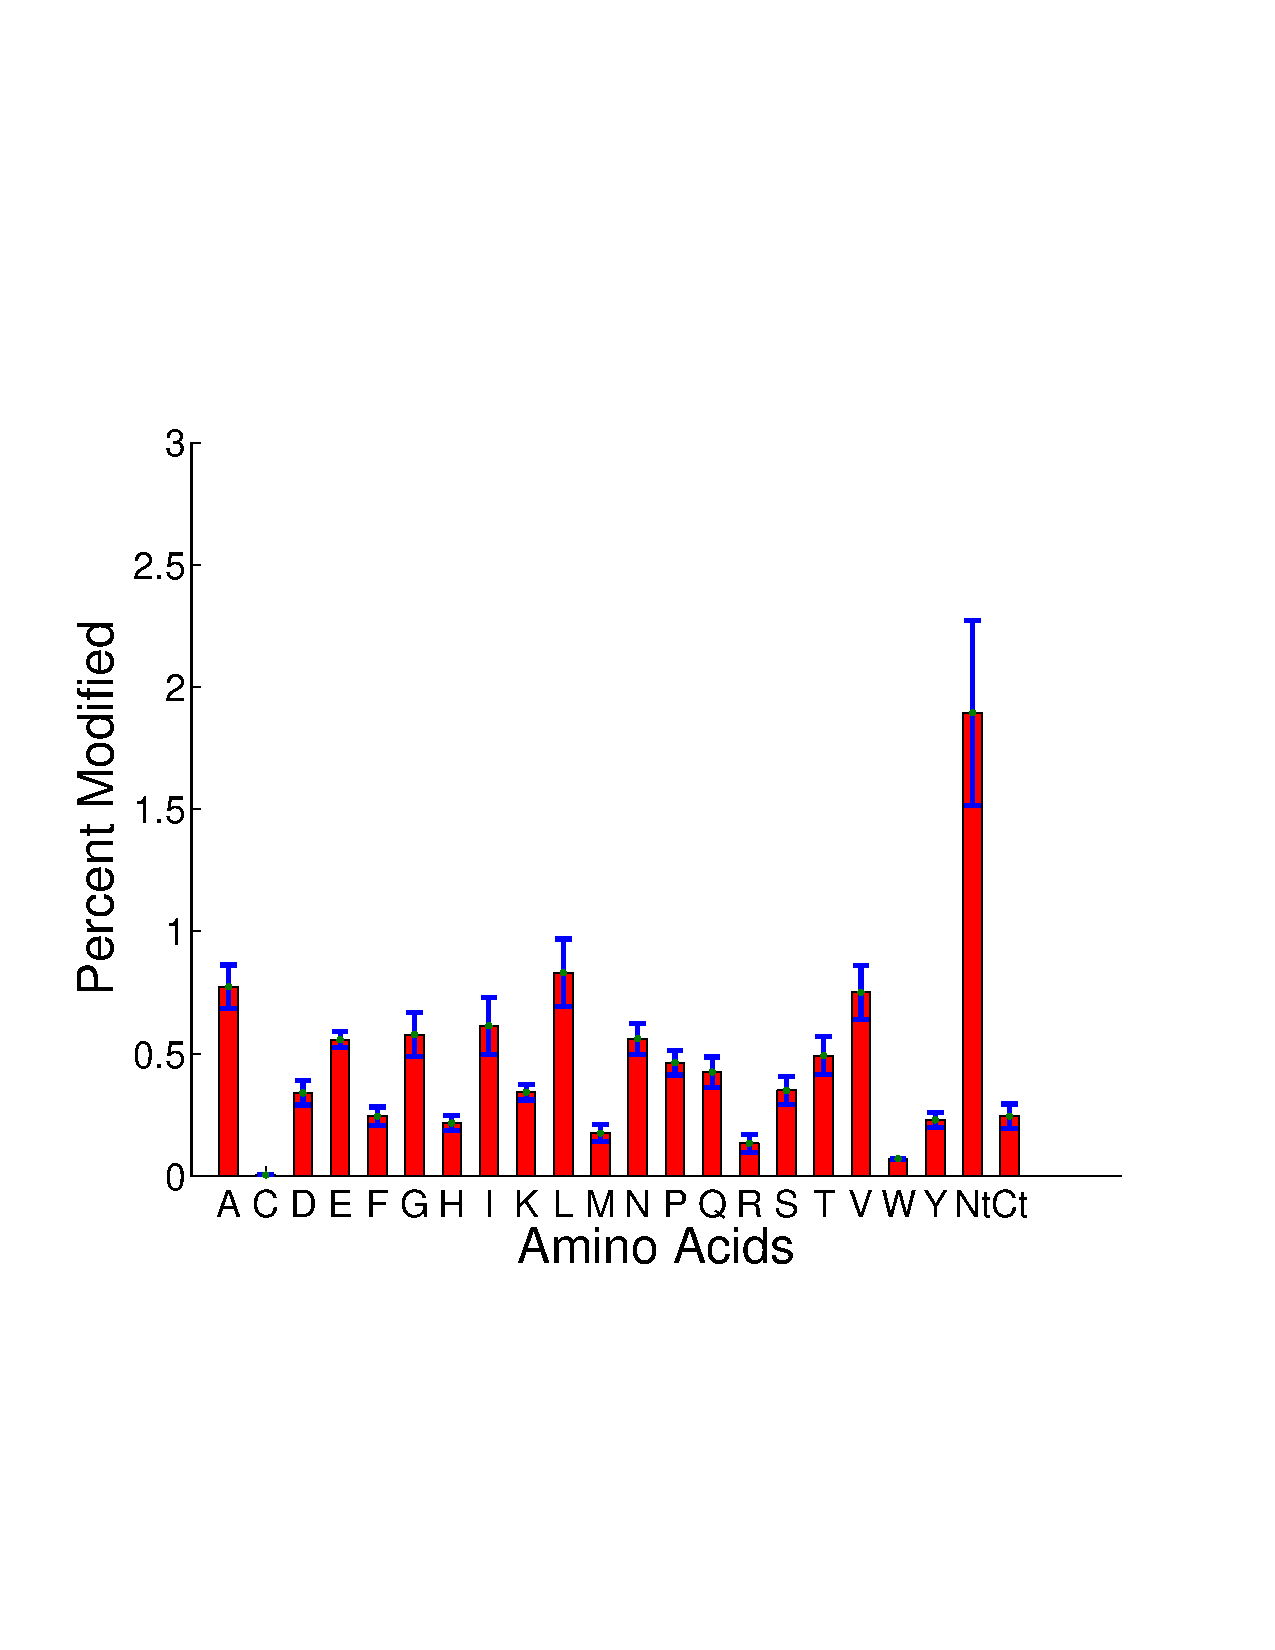
\includegraphics[width=5in]{Figures/1DaProfile.pdf}}
\customlabel{fig:1DaProfileFig}{S6}
\textbf{Figure S6: +1Da shift occurs randomly.} We cannot infer that this +1 Dalton mass-shift is deamidation as it occurs randomly on all amino acids, inferring it is carbon-13 (C13) peak picking as previously shown in many studies. 

\clearpage
\centerline{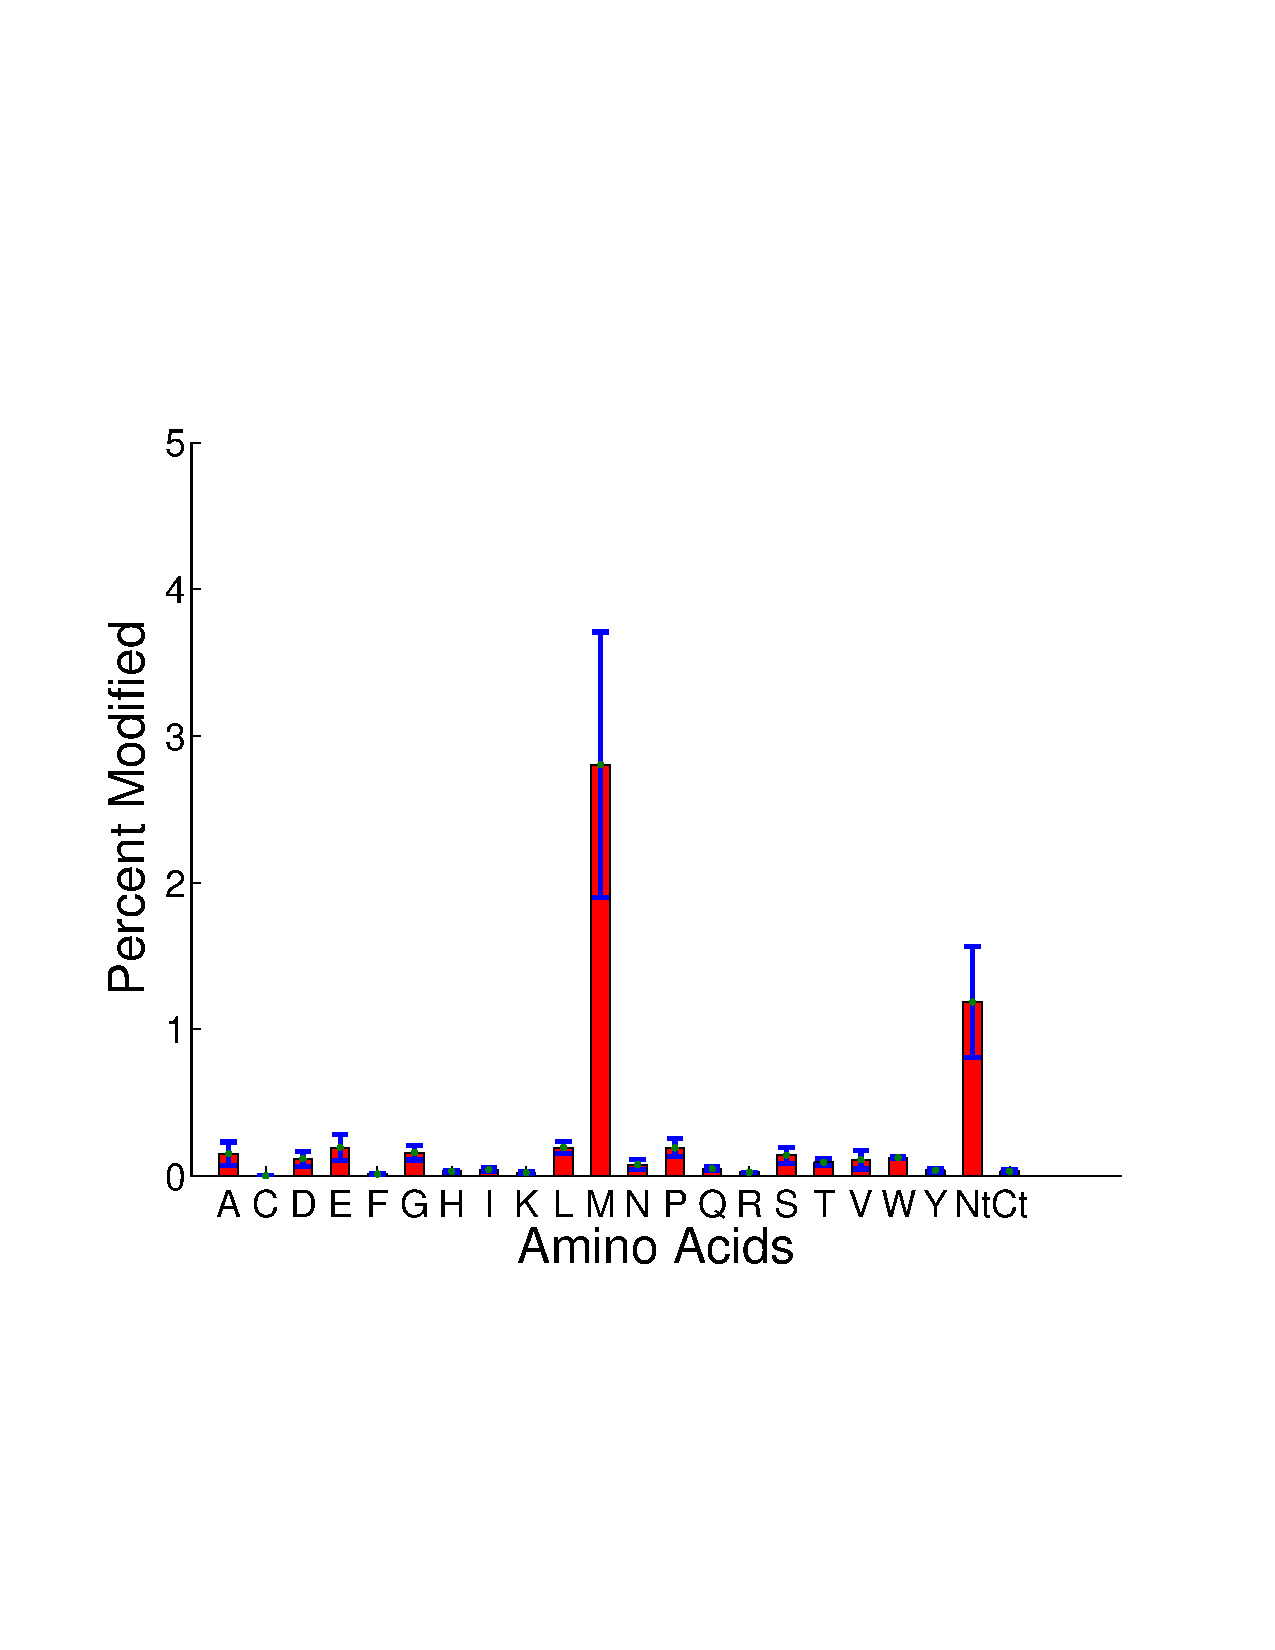
\includegraphics[width=5in]{Figures/OxidationProfile.pdf}}
\customlabel{fig:OxidationProfileFig}{S7}
\textbf{Figure S7: Oxidation is dominant on methionine.} Even though many amino acids could be oxidized, in this data set, oxidation seems to occur primarily on methionine, as expected. 

\clearpage
\centerline{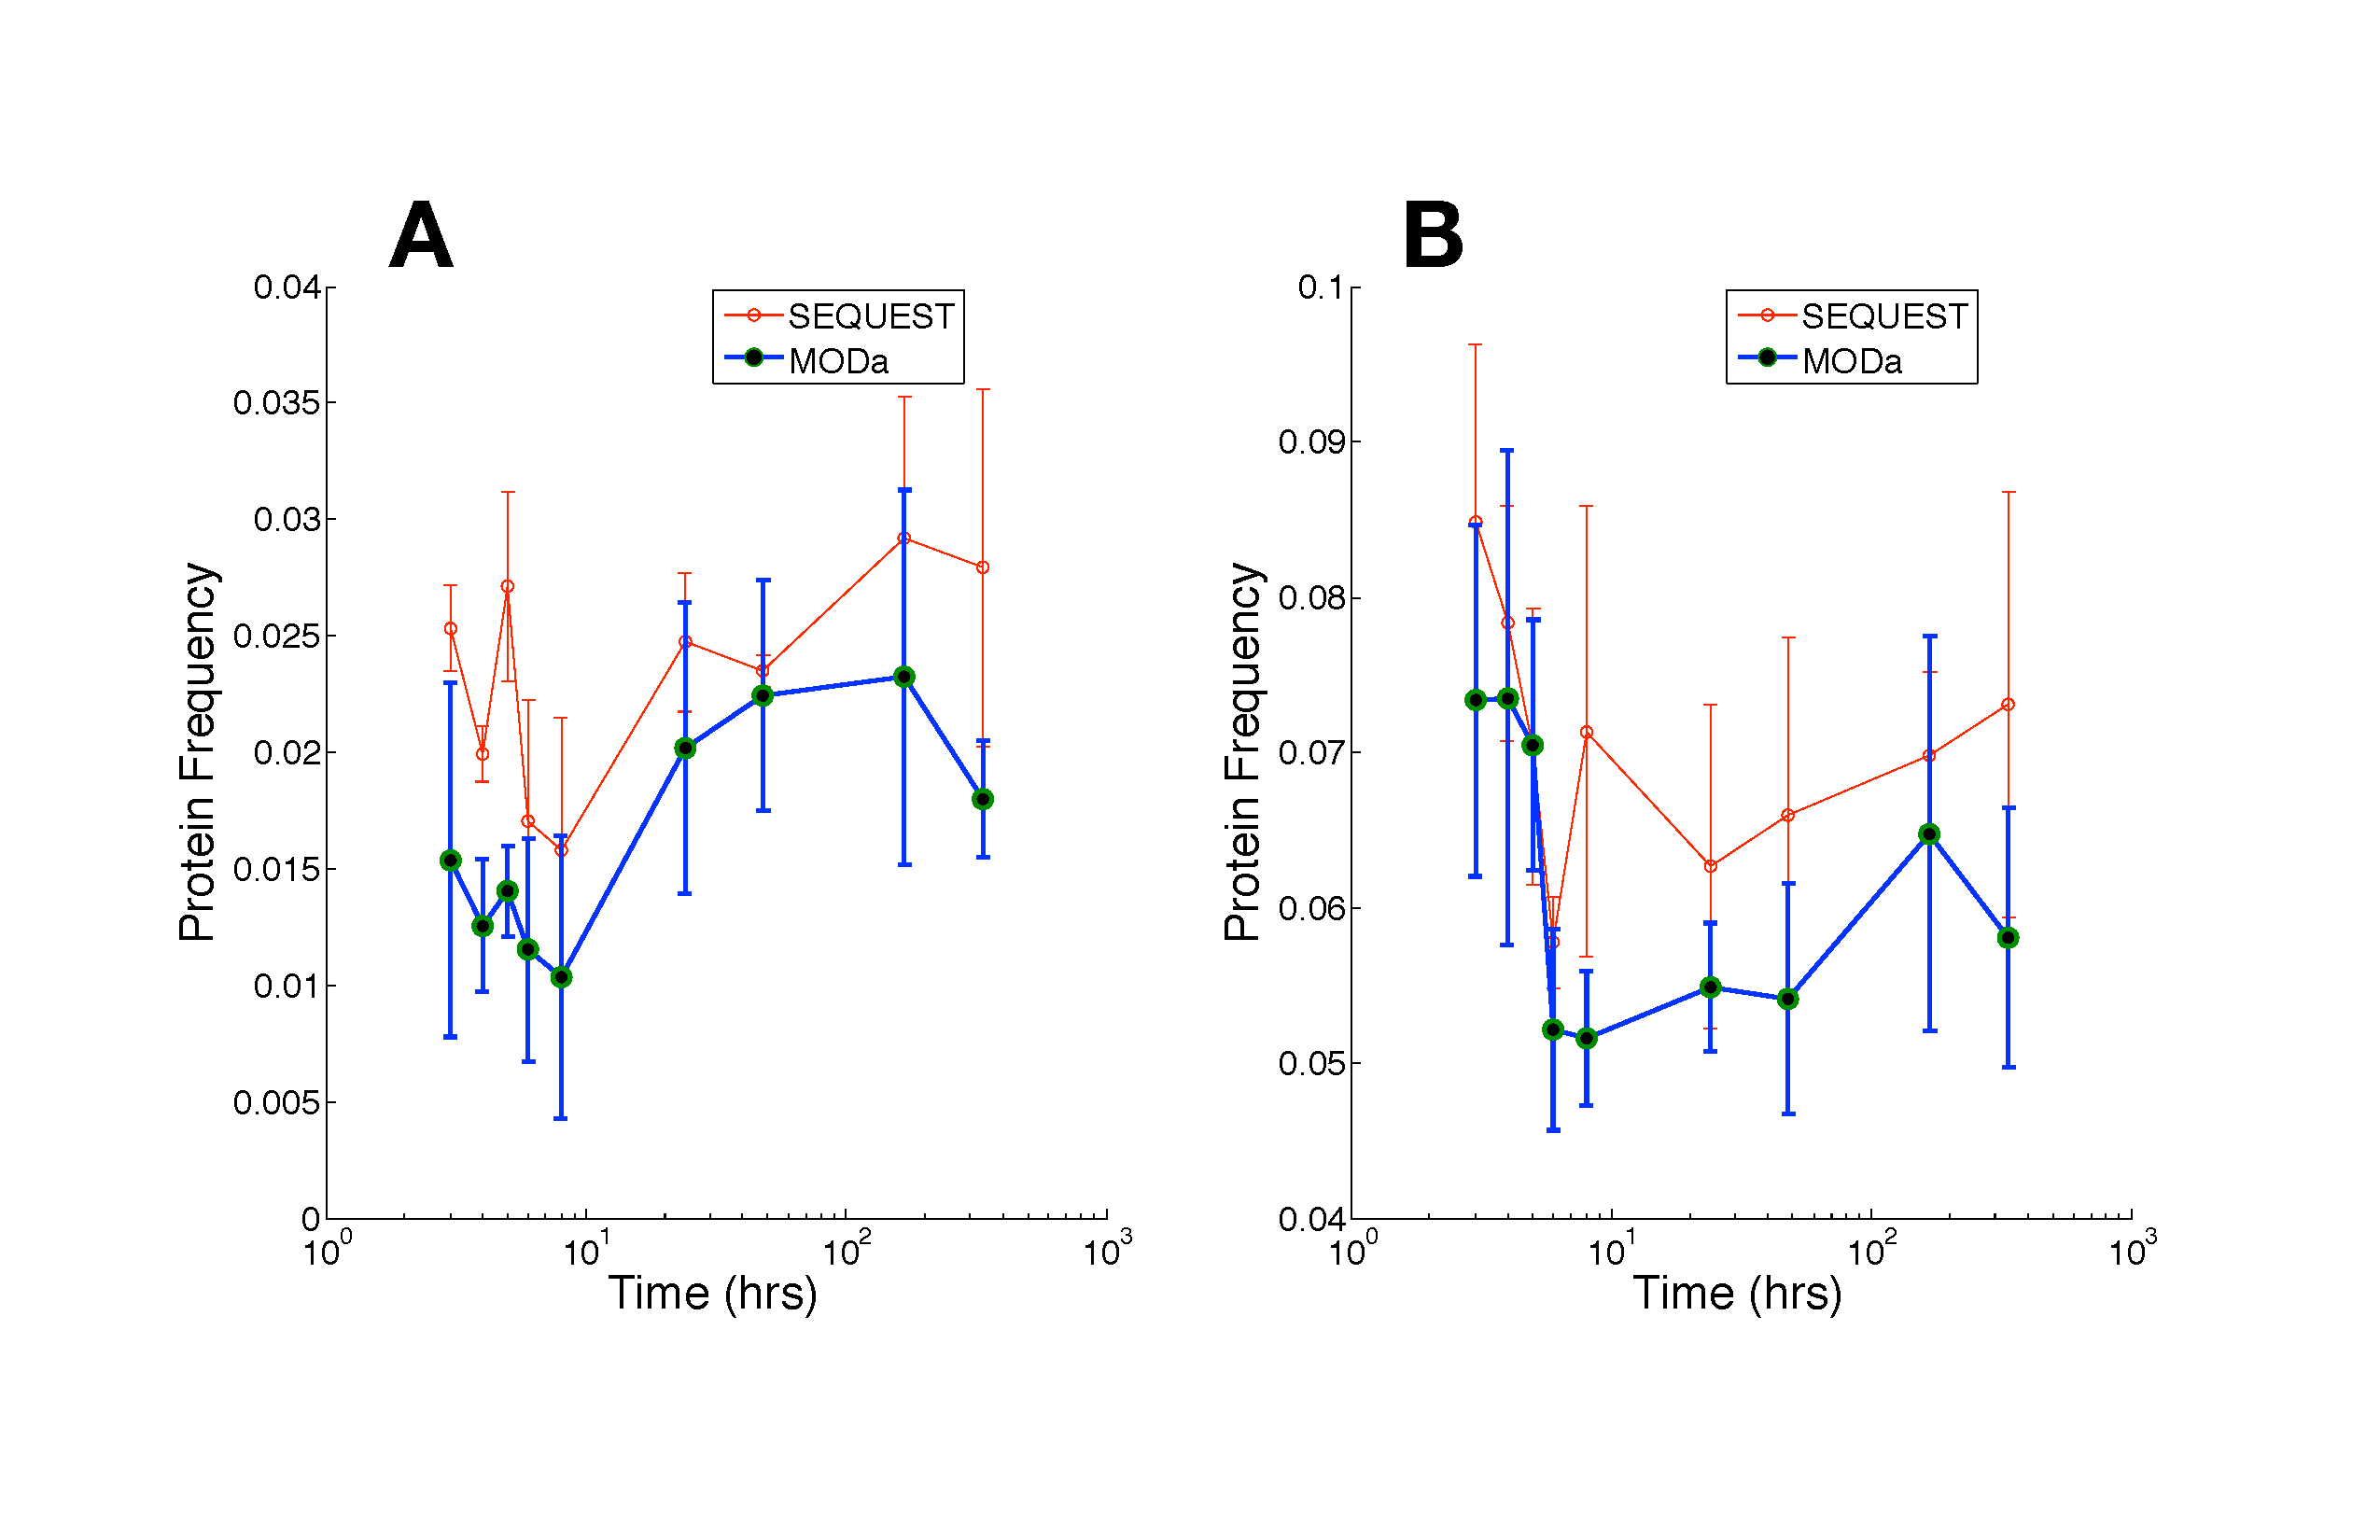
\includegraphics[width=8in]{Figures/Ecoli_MsrAB_MODa_Sequest.pdf}}
\customlabel{fig:SequestMODaFig}{S8}
\textbf{Figure S8: Sequest and MODa results agree.} We compared MODa protein abundance results with Sequest to double-check the protein levels of the sulfoxide reductases that protect \emph{E. coli} from oxidative stress by fixing MetSO to Met. As seen, MODa and Sequest results seem to agree well for (A) MsrA and (B) MsrB.

\clearpage
\centerline{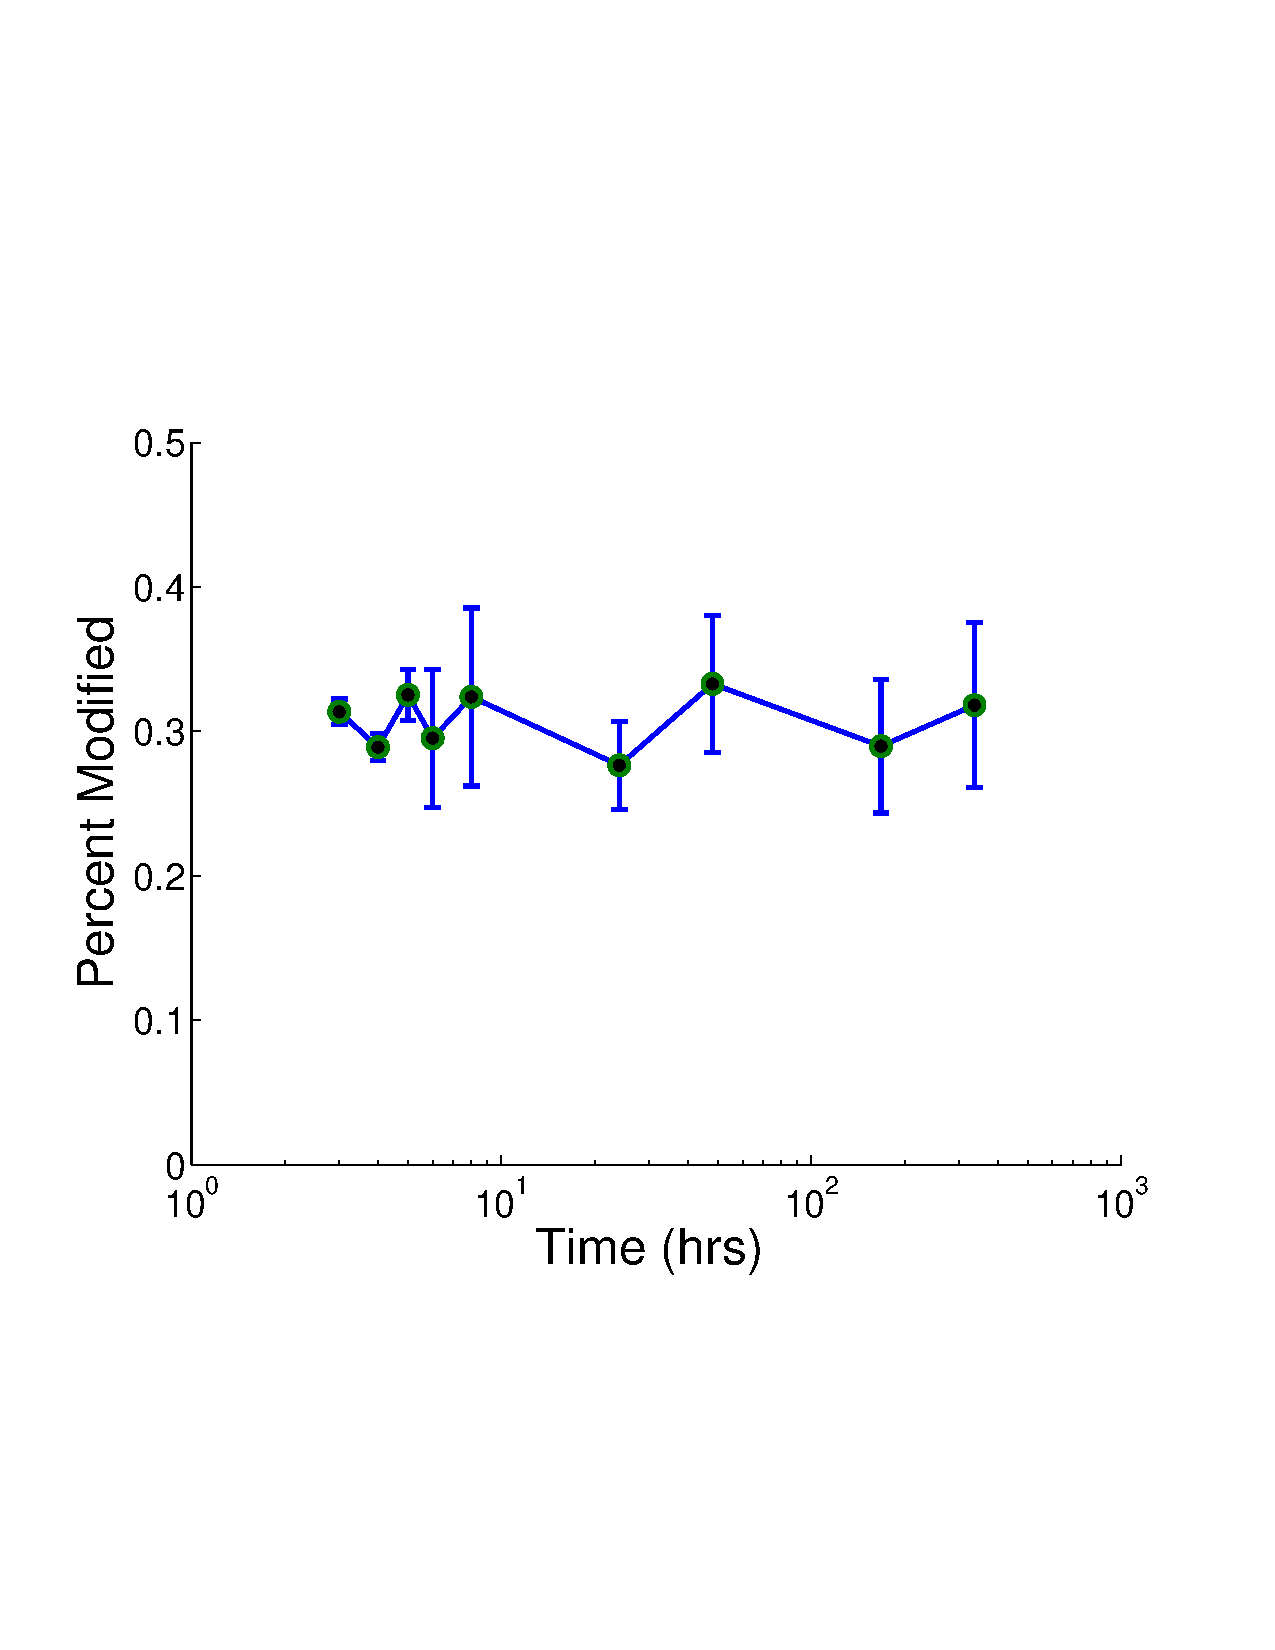
\includegraphics[width=5in]{Figures/PyroGlutamate.pdf}}
\customlabel{fig:PyroGlutamateFig}{S9}
\textbf{Figure S9: Glutamine to pyroglutamate conversion.} Glutamine to pyroglutamate happens to stabilize the protein. This conversion seems to be consistent across both the exponential and stationary phases. \textbf{\emph{Peptide pQ is artifact, protein N-terminal pQ is stabilizing.  Those cases need to be separated.}}

\clearpage
\centerline{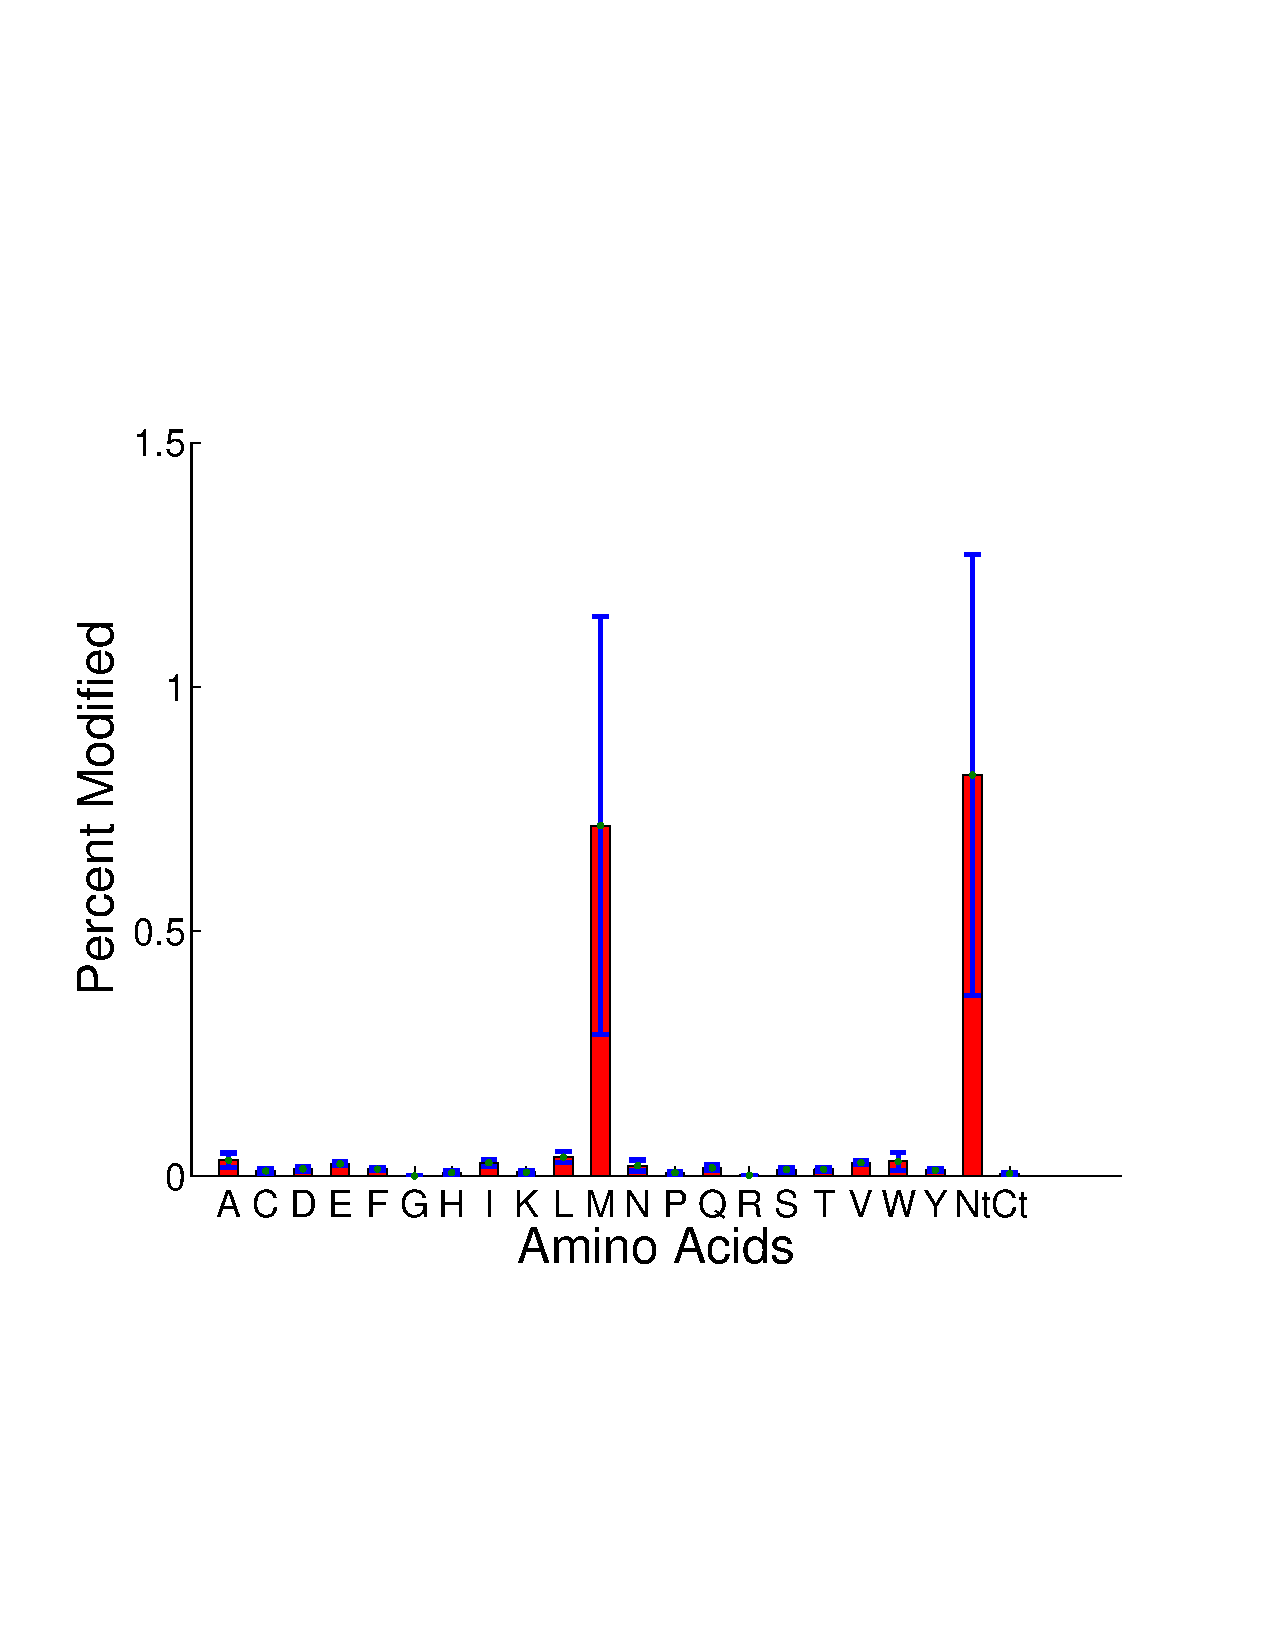
\includegraphics[width=5in]{Figures/MetGluProfile.pdf}}
\customlabel{fig:PyroGlutamateFig}{S10}
\textbf{Figure S10: Methionine to Glutamine subsitution.} Substitution ...

\section*{Supplementary Tables}
\customlabel{tab:mass_shifts}{S1}
\textbf{Table S1: .} These .
%\bigskip

\noindent File: \texttt{Figures/mS.csv}\\
%Available in github repository \texttt{https://github.com/clauswilke/Ecoli\_FBA\_input\_prediction}
\bigskip

%\end{table}



%\bigskip
%\customlabel{tab:predictive_nitrogen_sources}{S2}
%\noindent \textbf{Table S2: .} These .
%\bigskip

%\noindent File: \texttt{SupportingInfo/NitrogenSources.xlsx}\\
%Available in github repository \texttt{https://github.com/clauswilke/Ecoli\_FBA\_input\_prediction}

\end{document}
